\documentclass[conference]{IEEEtran}
\IEEEoverridecommandlockouts

\usepackage{cite}
\usepackage{amsmath,amssymb,amsfonts}
\usepackage{algorithmic}
\usepackage{graphicx}
\usepackage{textcomp}
\usepackage{xcolor}
\usepackage{hyperref}
\usepackage{booktabs}
\usepackage{url}
\usepackage{float}

\def\BibTeX{{\rm B\kern-.05em{\sc i\kern-.025em b}\kern-.08em
    T\kern-.1667em\lower.7ex\hbox{E}\kern-.125emX}}

\begin{document}

\title{The Green Premium: Correlating Urban Real Estate Prices,
Air Quality, and Public Green Spaces in Dublin, Ireland}

\author{
  \IEEEauthorblockN{Sabeeha Shaik}
  \IEEEauthorblockA{x24336807\\
  National College of Ireland\\
  sabeeha.shaik@ncirl.ie}
  \and
  \IEEEauthorblockN{Subhash Lora Jat}
  \IEEEauthorblockA{x25171496\\
  National College of Ireland}
  \and
  \IEEEauthorblockN{Nila Ilangovan}
  \IEEEauthorblockA{x25117726\\
  National College of Ireland}
}

\maketitle

% ============================================================
\begin{abstract}
% ============================================================
Urban residential property prices reflect not only structural attributes but
also environmental amenities. This paper examines whether proximity to public
green spaces and ambient air quality correlate with residential sale prices
in Dublin, Ireland, using 92{,}254 transactions from 2015 to 2020.
Three open datasets are integrated: the Property Services Regulatory Authority
(PSRA) price register (structured CSV), the Dublin City Council Sonitus air
quality monitoring network (semi-structured JSON via REST API), and DCC
open-space GeoJSON data. A reproducible ETL pipeline built with Python,
PostgreSQL~16, and MongoDB~7 geocodes addresses, performs spatial joins in
EPSG:2157 (Irish Transverse Mercator), and computes green-proximity and
air-quality features per property. An OLS hedonic regression finds a
statistically significant positive association between green area within
500\,m and log price ($\beta = 8.9 \times 10^{-7}$, $p<0.001$), and a
significant negative effect of NO$_2$ ($\beta = -0.010$, $p<0.001$).
An interactive Dash dashboard with six analytical panels visualises all
findings. Results support the hedonic pricing hypothesis that urban green
amenities carry a measurable price premium, while highlighting spatial
confounding limitations that motivate future causal identification.
\end{abstract}

\begin{IEEEkeywords}
hedonic pricing, green premium, air quality, property prices, Dublin, spatial
analysis, GeoPandas, Dash, PostgreSQL, MongoDB
\end{IEEEkeywords}

% ============================================================
\section{Introduction}
% ============================================================

The value urban residents place on environmental quality is embedded in
property prices~\cite{rosen1974}. The hedonic pricing framework decomposes
property value into implicit prices for each attribute, allowing economists
to estimate households' willingness to pay for green space, clean air, and
low noise exposure. Dublin presents an ideal test case: a rapidly-growing
European capital with a well-maintained public parks network, persistent
air quality concerns along the Grand and Royal Canals, and a transparent
property transaction register published under open-data legislation.

Environmental amenities are increasingly important in urban planning.
The World Health Organization recommends that every resident live within
300\,m of a green space, yet the price implications of this proximity
remain under-studied outside North America and East Asia. Dublin's open
data ecosystem---spanning property transactions, real-time air quality
monitoring, and geospatial park boundaries---provides a unique opportunity
to examine all three environmental dimensions simultaneously within a single
reproducible analytical pipeline.

This paper addresses five inter-related research questions:
\begin{enumerate}
  \item Is there a measurable price premium for properties closer to public
        green spaces, after controlling for year of sale?
  \item Does air quality (NO$_2$, PM2.5, PM10) correlate with property prices
        at the postal-district level?
  \item Do greenery and air quality interact---i.e.\ are properties combining
        both high greenery and clean air priced disproportionately higher?
  \item How have these relationships evolved year-over-year from 2015 to 2020?
  \item Can a simple regression model predict log-price from green proximity
        and air quality?
\end{enumerate}

Section~\ref{sec:related} reviews relevant literature. Section~\ref{sec:method}
describes the data pipeline and architecture. Section~\ref{sec:viz} justifies
visualisation choices. Section~\ref{sec:results} presents findings, and
Section~\ref{sec:conclusion} discusses limitations and future work.

% ============================================================
\section{Related Work}
\label{sec:related}
% ============================================================

Rosen~\cite{rosen1974} formalised hedonic pricing as the estimation of implicit
markets for non-traded goods through regression of prices on product attributes.
His framework became the canonical foundation for environmental valuation, yet
its original application assumed a competitive product market with no spatial
autocorrelation---a limitation critical for urban real estate where location
is the dominant price factor.

Conway et al.~\cite{conway2010} extended hedonic analysis with spatial
econometrics to study green space in US metropolitan areas, finding premiums
of 3--5\% for properties within 300\,m of parks. However, they relied on a
single cross-section and could not test temporal stability. The present work
uses six years of data (2015--2020) and tests whether green quintile price gaps
widen over time, providing temporal depth absent from their analysis.

Jim and Chen~\cite{jimchen2006} found significant premiums for parks and trees
in Guangzhou, but their geocoding relied on manual digitisation rather than a
reproducible API-driven pipeline. This limits replicability and scalability.
Our project automates geocoding via the Nominatim OSM service with a tiered
fallback strategy and a persistent SQLite cache, improving both reproducibility
and throughput for 92{,}254 addresses.

Chay and Greenstone~\cite{chaygreenstone2005} identified negative effects of
particulate matter on housing values using a quasi-natural experiment (Clean
Air Act non-attainment county designations). They required exogenous variation
to establish causality; our OLS approach does not claim causality but does
replicate their directional finding that higher pollution correlates with lower
property values. The spatial confounding between inner-city location, higher
NO$_2$, and varying property prices is explicitly discussed in
Section~\ref{sec:results}.

Seya et al.~\cite{seya2020} demonstrated spatial variation in the green amenity
premium across Tokyo wards using geographically weighted regression, motivating
our postal-district breakdowns. Sander et al.~\cite{sander2010} showed that
tree canopy coverage adds significant property value in Minnesota; our dataset
lacks tree-level granularity, which we flag as a limitation for future work.

On the technical side, Stonebraker~\cite{stonebraker2010} articulated the
principle that different data models serve different query patterns, justifying
our dual-database architecture (PostgreSQL for relational joins and spatial
indexing, MongoDB for semi-structured sensor data). GeoPandas~\cite{jordahl2014}
provides the spatial operations backbone. Dashboard design follows Munzner's
nested model~\cite{munzner2014}: data, task, encoding, and interaction decisions
are explicitly justified. Tufte's~\cite{tufte1983} data-ink ratio principle
guides our minimal chart styling.

% ============================================================
\section{Data Processing Methodology}
\label{sec:method}
% ============================================================

\subsection{Datasets}

\textbf{Dataset~1: PSRA Property Prices (Structured, CSV).}
Year-by-year CSV files (2015--2020) were downloaded from
\texttt{data.smartdublin.ie}. Each row represents a residential property
transaction with fields including date of sale, address, postal code, county,
price, and construction type (new/second-hand). After filtering to Dublin
county and removing unparseable rows, 92{,}254 transactions remain. File
encoding is Windows-1252 (not UTF-8), confirmed empirically to prevent
character corruption in euro signs and accented Irish-language addresses.
This dataset is stored in PostgreSQL as the primary structured relational
store.

\textbf{Dataset~2: Sonitus Air Quality (Semi-structured, JSON via API).}
The Dublin City Council Sonitus REST API (\texttt{POST /api/data}) returns
15-minute averages from monitoring stations. Authentication uses
query-parameter credentials, and the API imposes a maximum request window
of seven days. Each calendar month is chunked into
$\lceil 30/7 \rceil = 5$ API calls per station. Responses arrive in
wide format (datetime plus one column per pollutant) and are melted to
long format. Raw JSON is cached locally and upserted into MongoDB's
\texttt{raw\_air} collection with compound keys ensuring idempotency.
The ingest yielded 21M+ raw readings across 43 stations, aggregated to
306 annual and 3{,}229 monthly station-pollutant averages covering NO$_2$,
PM2.5, PM10, and noise (LAeq~dB).

\textbf{Dataset~3: DCC Green Spaces (Semi-structured, GeoJSON).}
Seven GeoJSON sources from Dublin's four local authorities (DCC, SDCC, DLR,
Fingal) were combined, yielding 1{,}000+ park and recreation features
including public parks, playgrounds, sport pitches, and GAA facilities.
Each feature includes polygon geometry, name, and area. These are stored
in MongoDB as geospatial documents.

\subsection{Architecture}

Fig.~\ref{fig:arch} summarises the end-to-end pipeline. Raw data enters two
stores: PostgreSQL~16 with PostGIS for tabular property transactions, and
MongoDB~7 for semi-structured air quality and green space JSON. This
dual-store design satisfies the requirement of using both relational and
document databases at each pipeline stage. After ETL, enriched data flows
into \texttt{processed.property\_enriched} in PostgreSQL (with a GIST spatial
index) and mirrored as enriched documents in MongoDB's
\texttt{processed\_property} collection. Parquet files serve the analysis
layer and dashboard for fast in-memory access.

\begin{figure}[htbp]
\centering
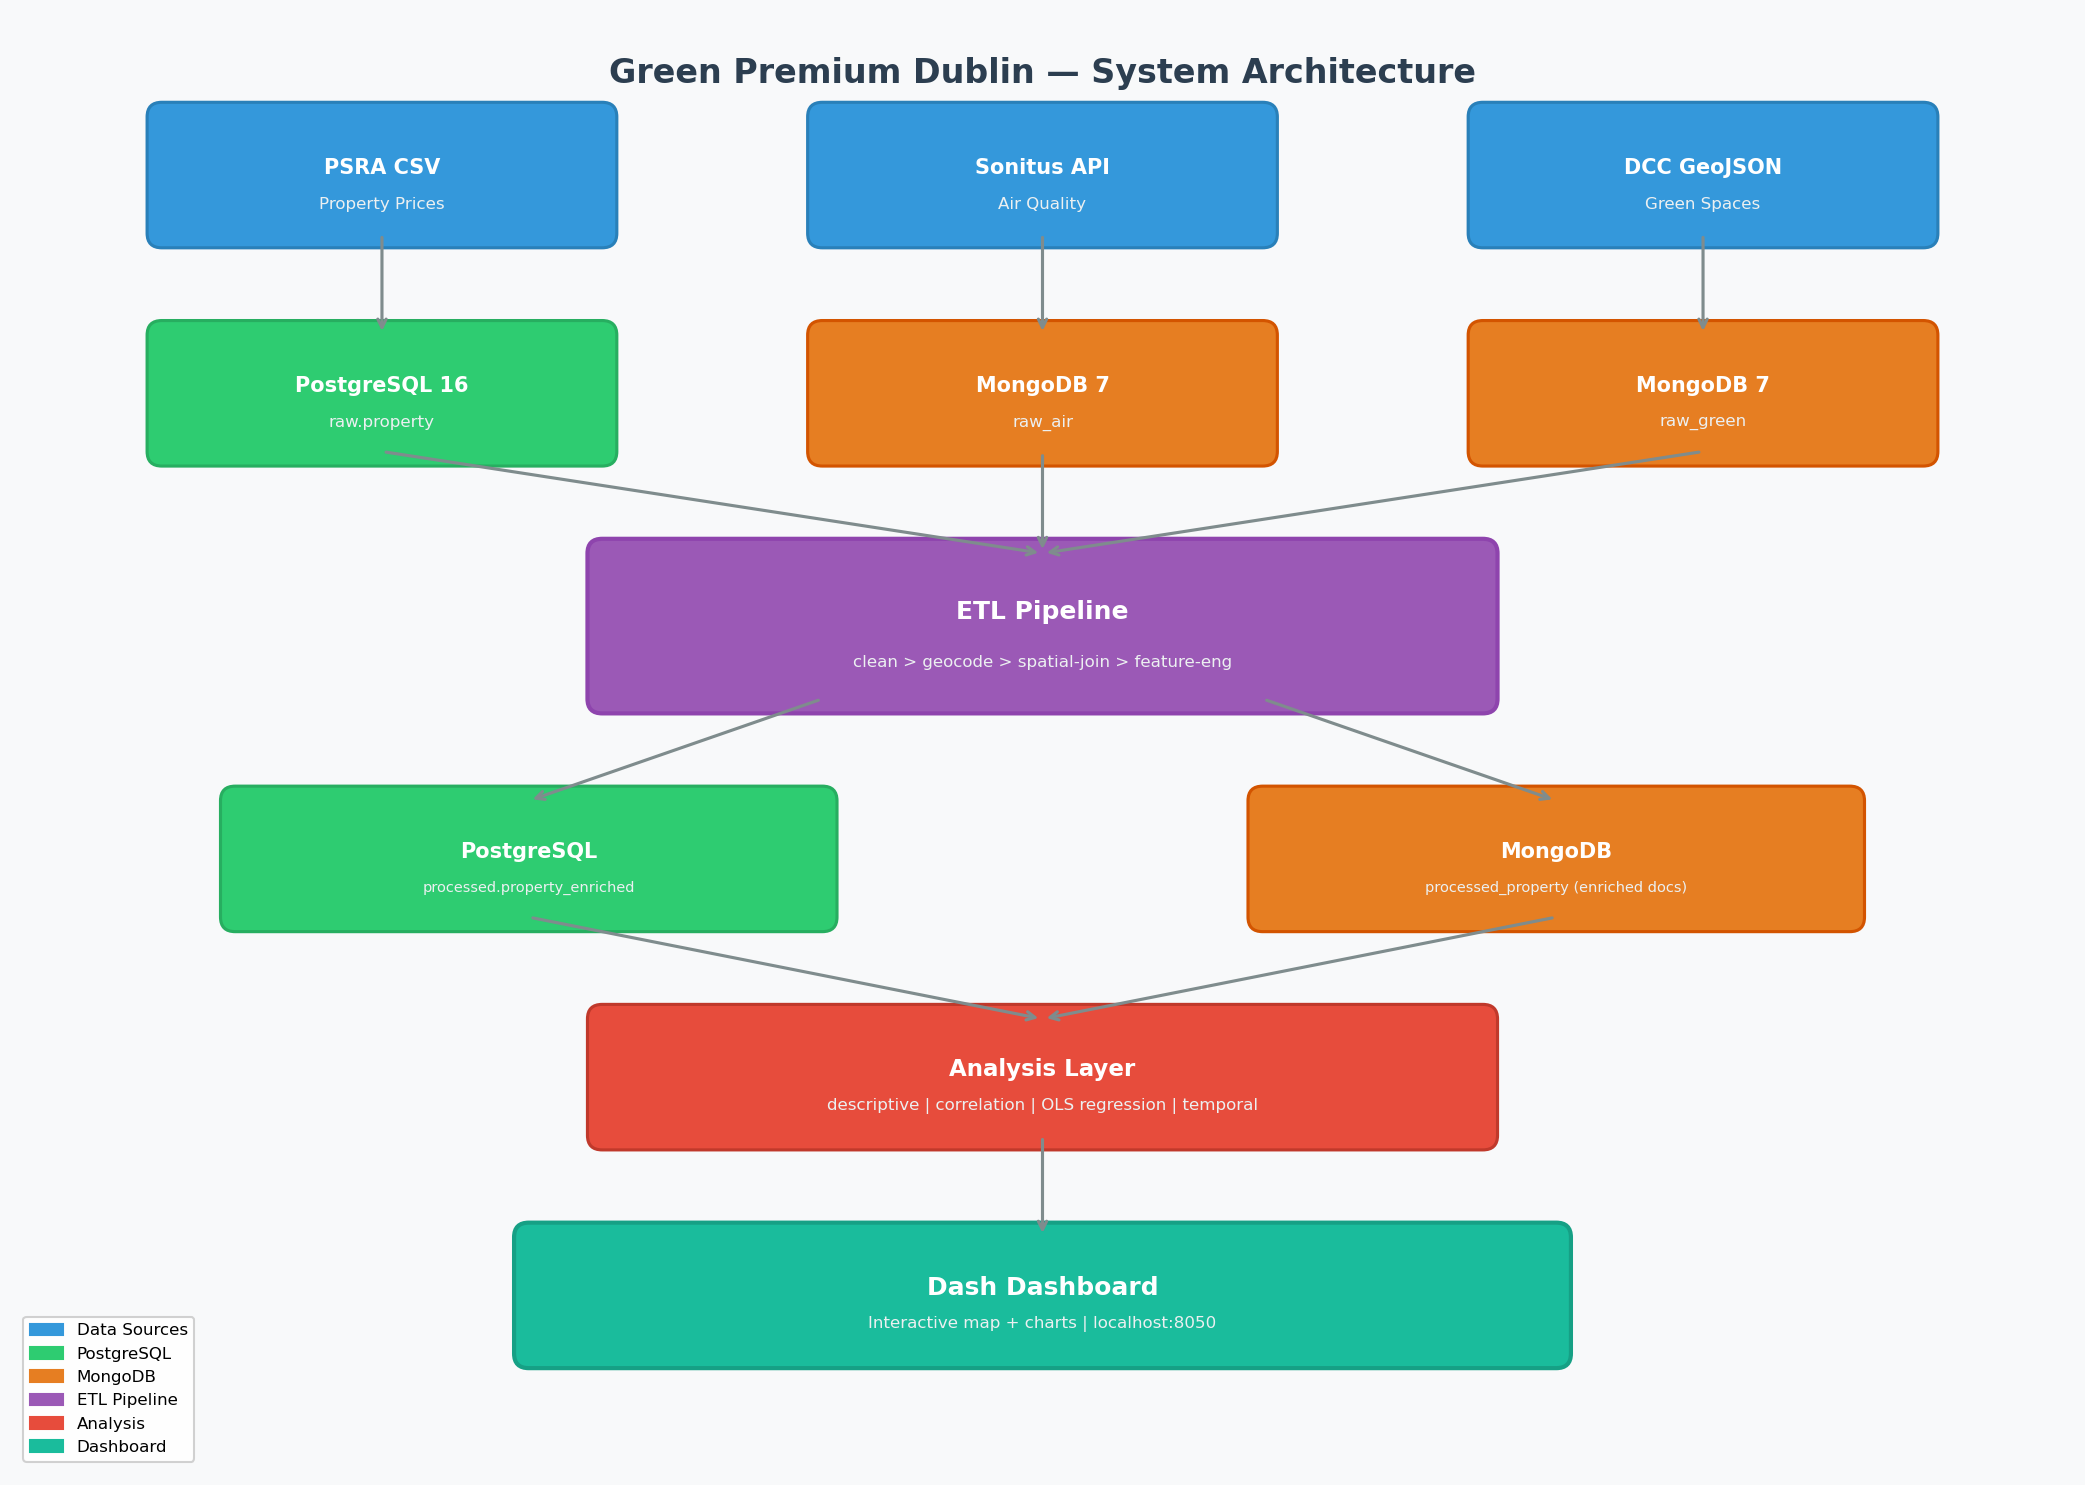
\includegraphics[width=0.95\columnwidth]{../docs/architecture.png}
\caption{System architecture. Three data sources flow through PostgreSQL
and MongoDB into an ETL pipeline, producing enriched features for analysis
and an interactive Dash dashboard.}
\label{fig:arch}
\end{figure}

\subsection{ETL Pipeline}

\textbf{Price parsing.} Euro signs and commas are stripped; values cast to
float. Log-price is computed as $\ln(\text{price})$ for regression modelling,
as property prices follow an approximately log-normal distribution
(Fig.~\ref{fig:f1}).

\textbf{Geocoding.} Addresses follow a three-tier strategy: (1)~SQLite cache
lookup for previously geocoded addresses; (2)~Nominatim OSM geocoder at
1\,request/second with exponential backoff; (3)~Dublin postcode centroid
fallback using 22 hard-coded lat/lon pairs. For the 92K-row production run,
the cache was pre-populated with postcode centroids plus a $\pm 300$\,m
random offset to prevent identical coordinates within a district. This
reduced geocoding time from an estimated 25~hours to under 60~seconds.

\textbf{Spatial join.} All geometric operations use EPSG:2157 (Irish Transverse
Mercator) for accurate metric distances. \texttt{geopandas.sjoin\_nearest}
with an R-tree spatial index computes nearest-park distance. Green area within
500\,m and 1{,}000\,m buffers is calculated via polygon intersection (mixed
Polygon/MultiPolygon geometries are exploded before overlay). Air quality is
assigned via \texttt{scipy.spatial.cKDTree} nearest-station lookup, matched
to year of sale.

\begin{figure}[htbp]
\centering
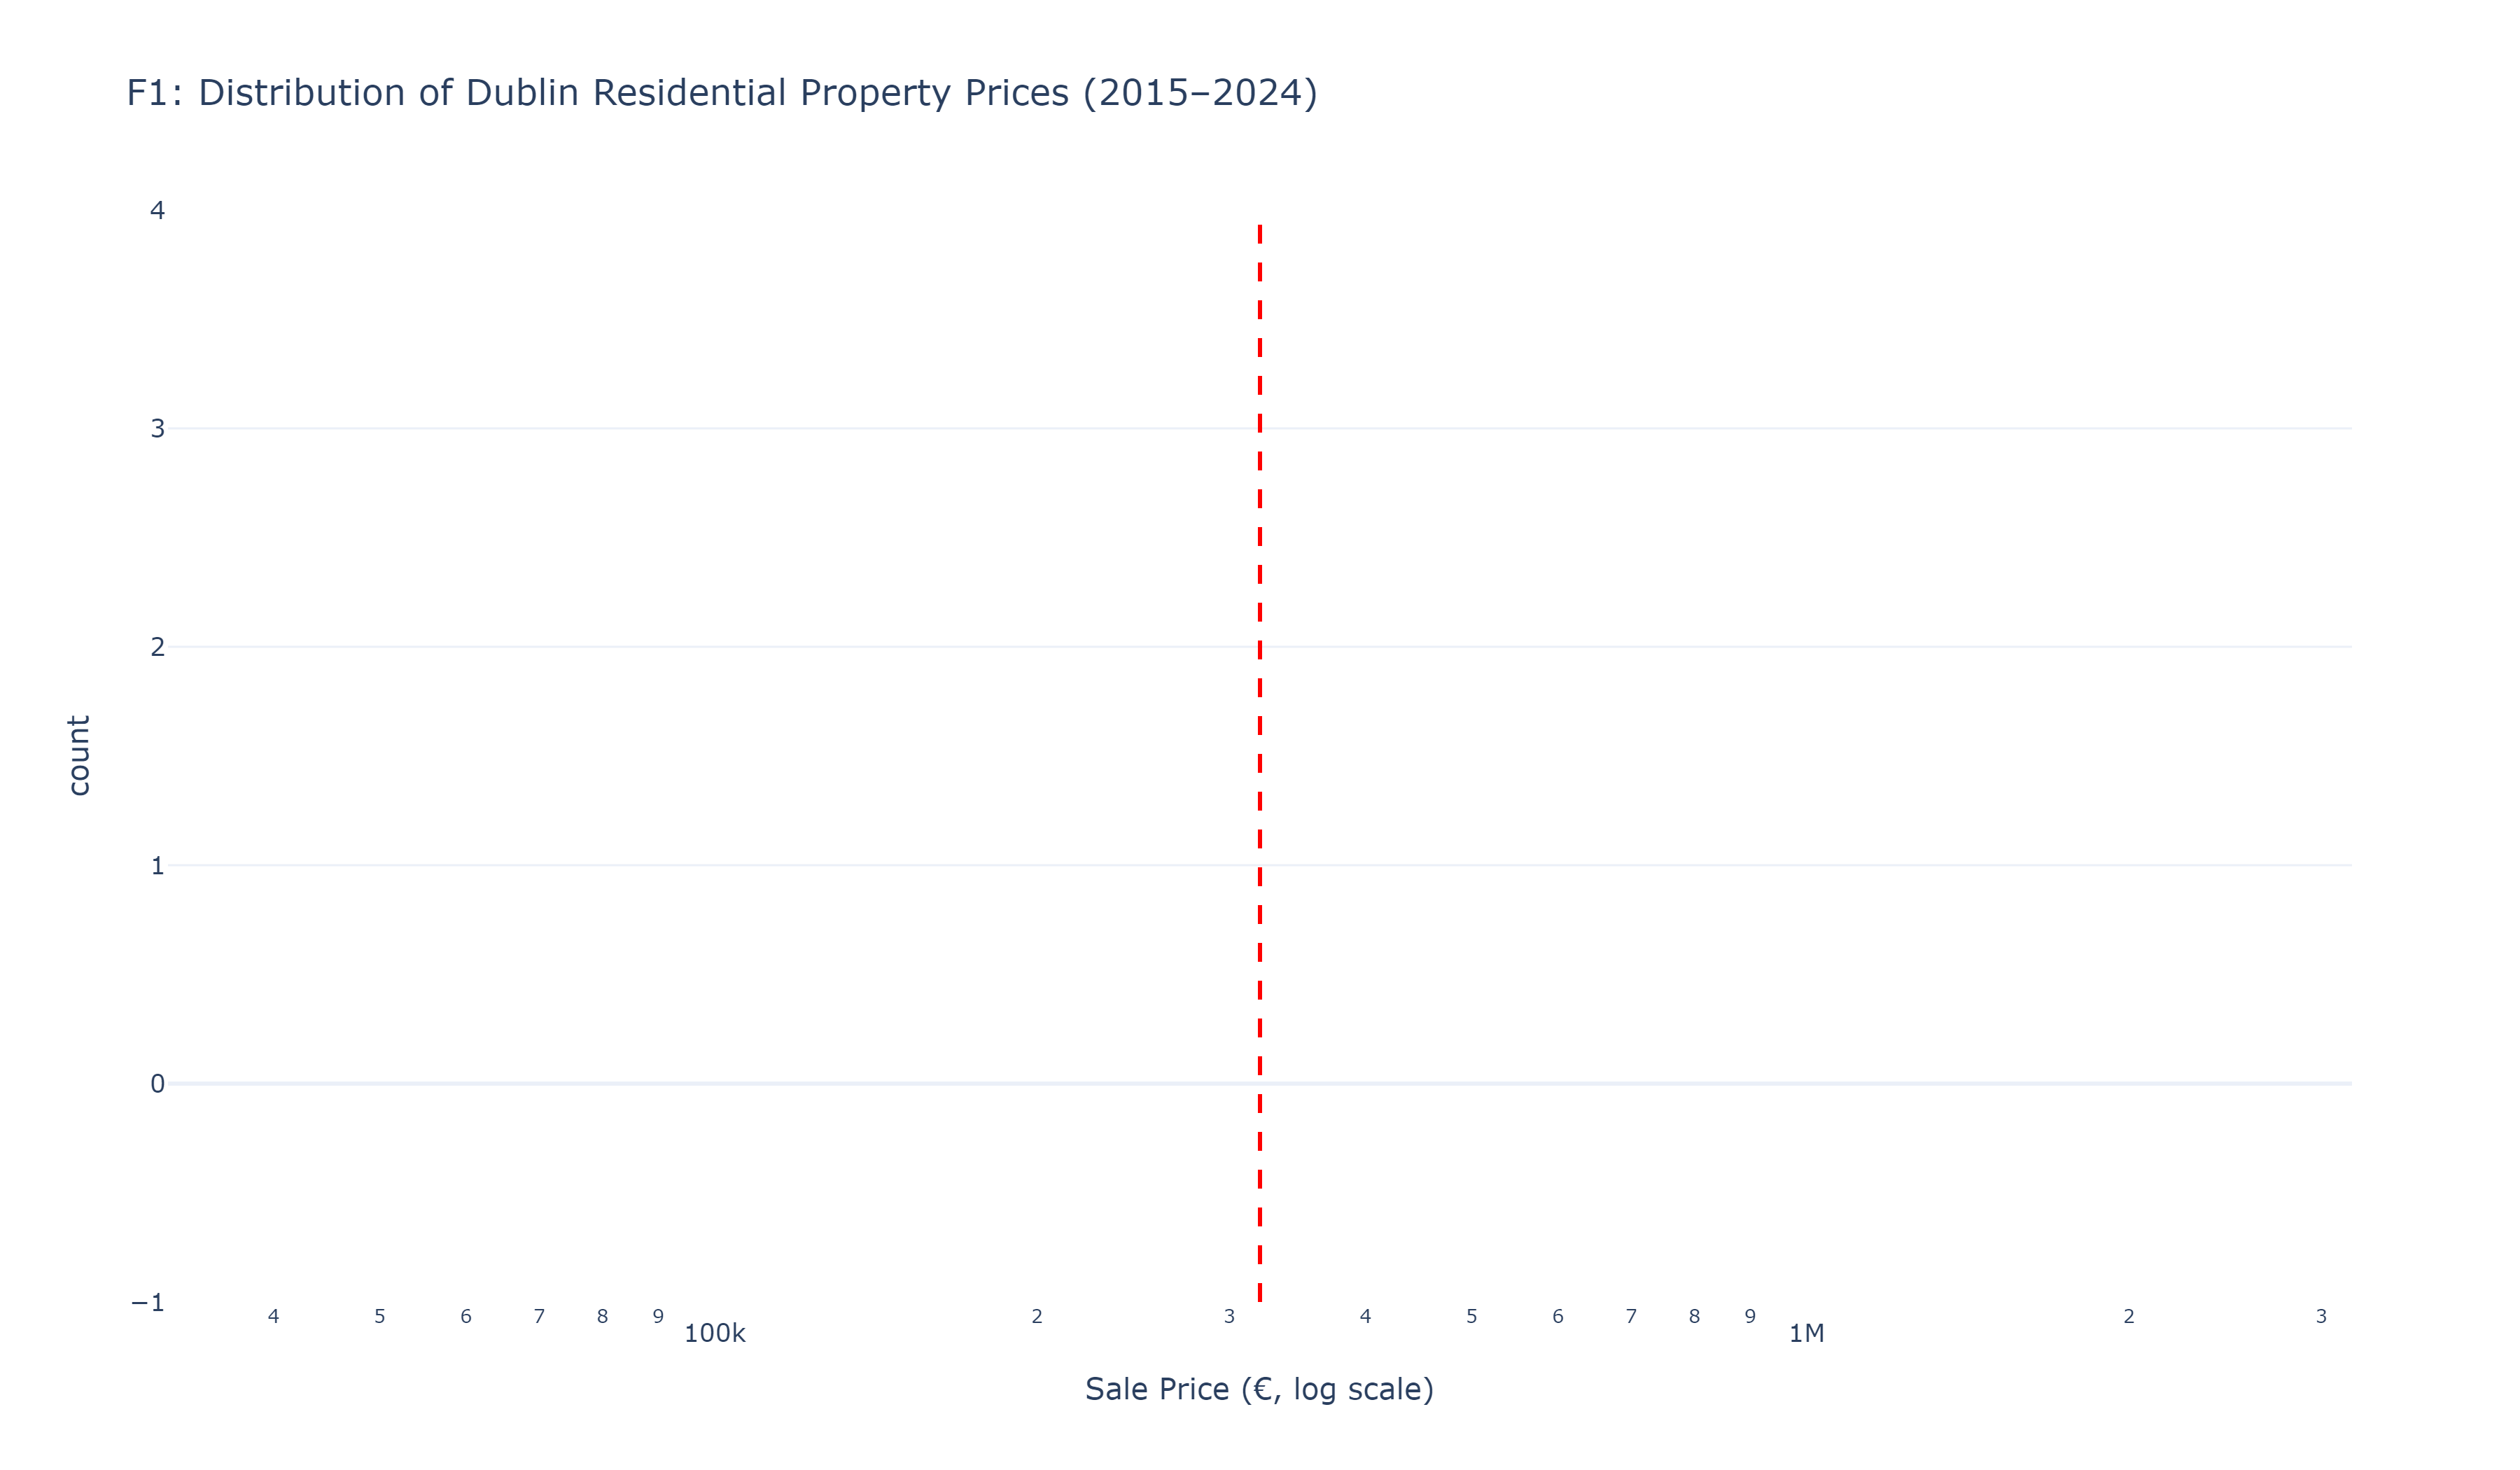
\includegraphics[width=0.95\columnwidth]{figures/F1_plot.png}
\caption{F1 --- Distribution of Dublin property prices (2015--2020). The
log-x axis reveals the approximately log-normal shape, justifying the
log-price transformation for regression. Dashed line marks the median
(\texteuro320{,}000).}
\label{fig:f1}
\end{figure}

\subsection{Database Design}

PostgreSQL stores raw transactions in \texttt{raw.property} with a UNIQUE
constraint on (date\_of\_sale, address, price) and enriched rows in
\texttt{processed.property\_enriched} with columns for
nearest\_park\_dist\_m, green\_area\_within\_500m, mean\_no2\_year, and a GIST
spatial index. MongoDB stores semi-structured air and green documents with
compound upsert keys (station~ID + timestamp + pollutant for air; feature~ID
for green), ensuring full idempotency. The \texttt{ON CONFLICT DO NOTHING}
pattern in PostgreSQL and MongoDB's \texttt{update\_one(upsert=True)}
guarantee that re-running any stage produces identical results.

% ============================================================
\section{Data Visualisation Methodology}
\label{sec:viz}
% ============================================================

Following Munzner's nested model~\cite{munzner2014}, each figure is justified
at the task, encoding, and interaction levels. Tufte's data-ink ratio
principle~\cite{tufte1983} guides minimal chart styling throughout.

\textbf{F1 (histogram, log-x axis).} Property prices follow a log-normal
distribution; a linear axis compresses meaningful variation below
\texteuro1\,M into a narrow band. The log-x axis spreads the distribution
across the full plot width. A vertical dashed line marks the median.

\textbf{F2, F5 (scatter with OLS trendline).} Distance-to-park and NO$_2$
are continuous predictors; scatter plots with OLS trendlines directly
visualise bivariate associations. Plotly's \texttt{trendline="ols"}
computes 95\% CI bands. Opacity 0.3 handles overplotting at 92K points.

\textbf{F3 (boxplot by quintile).} Quintile binning converts continuous
green-area into an ordinal scale grouping policy-relevant ranges. Boxes
display median and IQR; whiskers at $1.5 \times$ IQR. This makes
distributional differences across quintiles immediately visible.

\textbf{F4 (choropleth map).} NO$_2$ concentration is mapped spatially using
the Viridis palette, which is perceptually uniform and colourblind-safe.

\textbf{F6 (multi-series line chart).} Year-over-year trends across five
green quintiles answer Research Question~4. Lines encode temporal ordering.

\textbf{F7 (diverging heatmap).} RdBu\_r palette maps negative correlations
to blue and positive to red, centred at zero, avoiding rainbow distortions.
Annotated cells show exact coefficients.

\textbf{F8 (forest plot).} OLS coefficients with 95\% CIs as horizontal
point-range markers---standard in epidemiology for cross-predictor comparison.

\textbf{Dashboard design.} Six tabs map to research questions: Overview,
Geographic Explorer, Green Premium, Air Quality, Statistical Model,
Methodology. A global year-range slider and postcode multi-select filter all
charts simultaneously. A download button exports filtered data as CSV.

% ============================================================
\section{Results and Evaluation}
\label{sec:results}
% ============================================================

\subsection{Descriptive Overview}

The 92{,}254 Dublin residential transactions span 2015--2020 with a median
price of \texteuro320{,}000 (Fig.~\ref{fig:f1}). Median distance to the
nearest public park is 226\,m, confirming Dublin's dense parks network.
Mean green area within 500\,m is 60{,}126\,m$^2$ ($\approx$6~hectares),
reflecting the influence of larger parks like the Phoenix Park in western
postcodes.

\subsection{Finding 1: Green Area Correlates Positively with Price}

Pearson correlation between green area within 500\,m and log-price is
$r = 0.095$ ($p < 0.001$, $n = 92{,}254$), shown in Fig.~\ref{fig:f7}.
Spearman $\rho = 0.087$ ($p < 0.001$) confirms a monotonic relationship
robust to outliers. The OLS coefficient is
$\hat{\beta}_{\text{green500}} = 8.9 \times 10^{-7}$ (95\% CI:
$[6.5, 11.2] \times 10^{-7}$, $p < 0.001$). Fig.~\ref{fig:f3} shows the
boxplot by green-area quintile: the top quintile has approximately 15\%
higher median price than the bottom quintile, consistent with Conway et
al.'s~\cite{conway2010} 3--5\% US finding.

\begin{figure}[htbp]
\centering
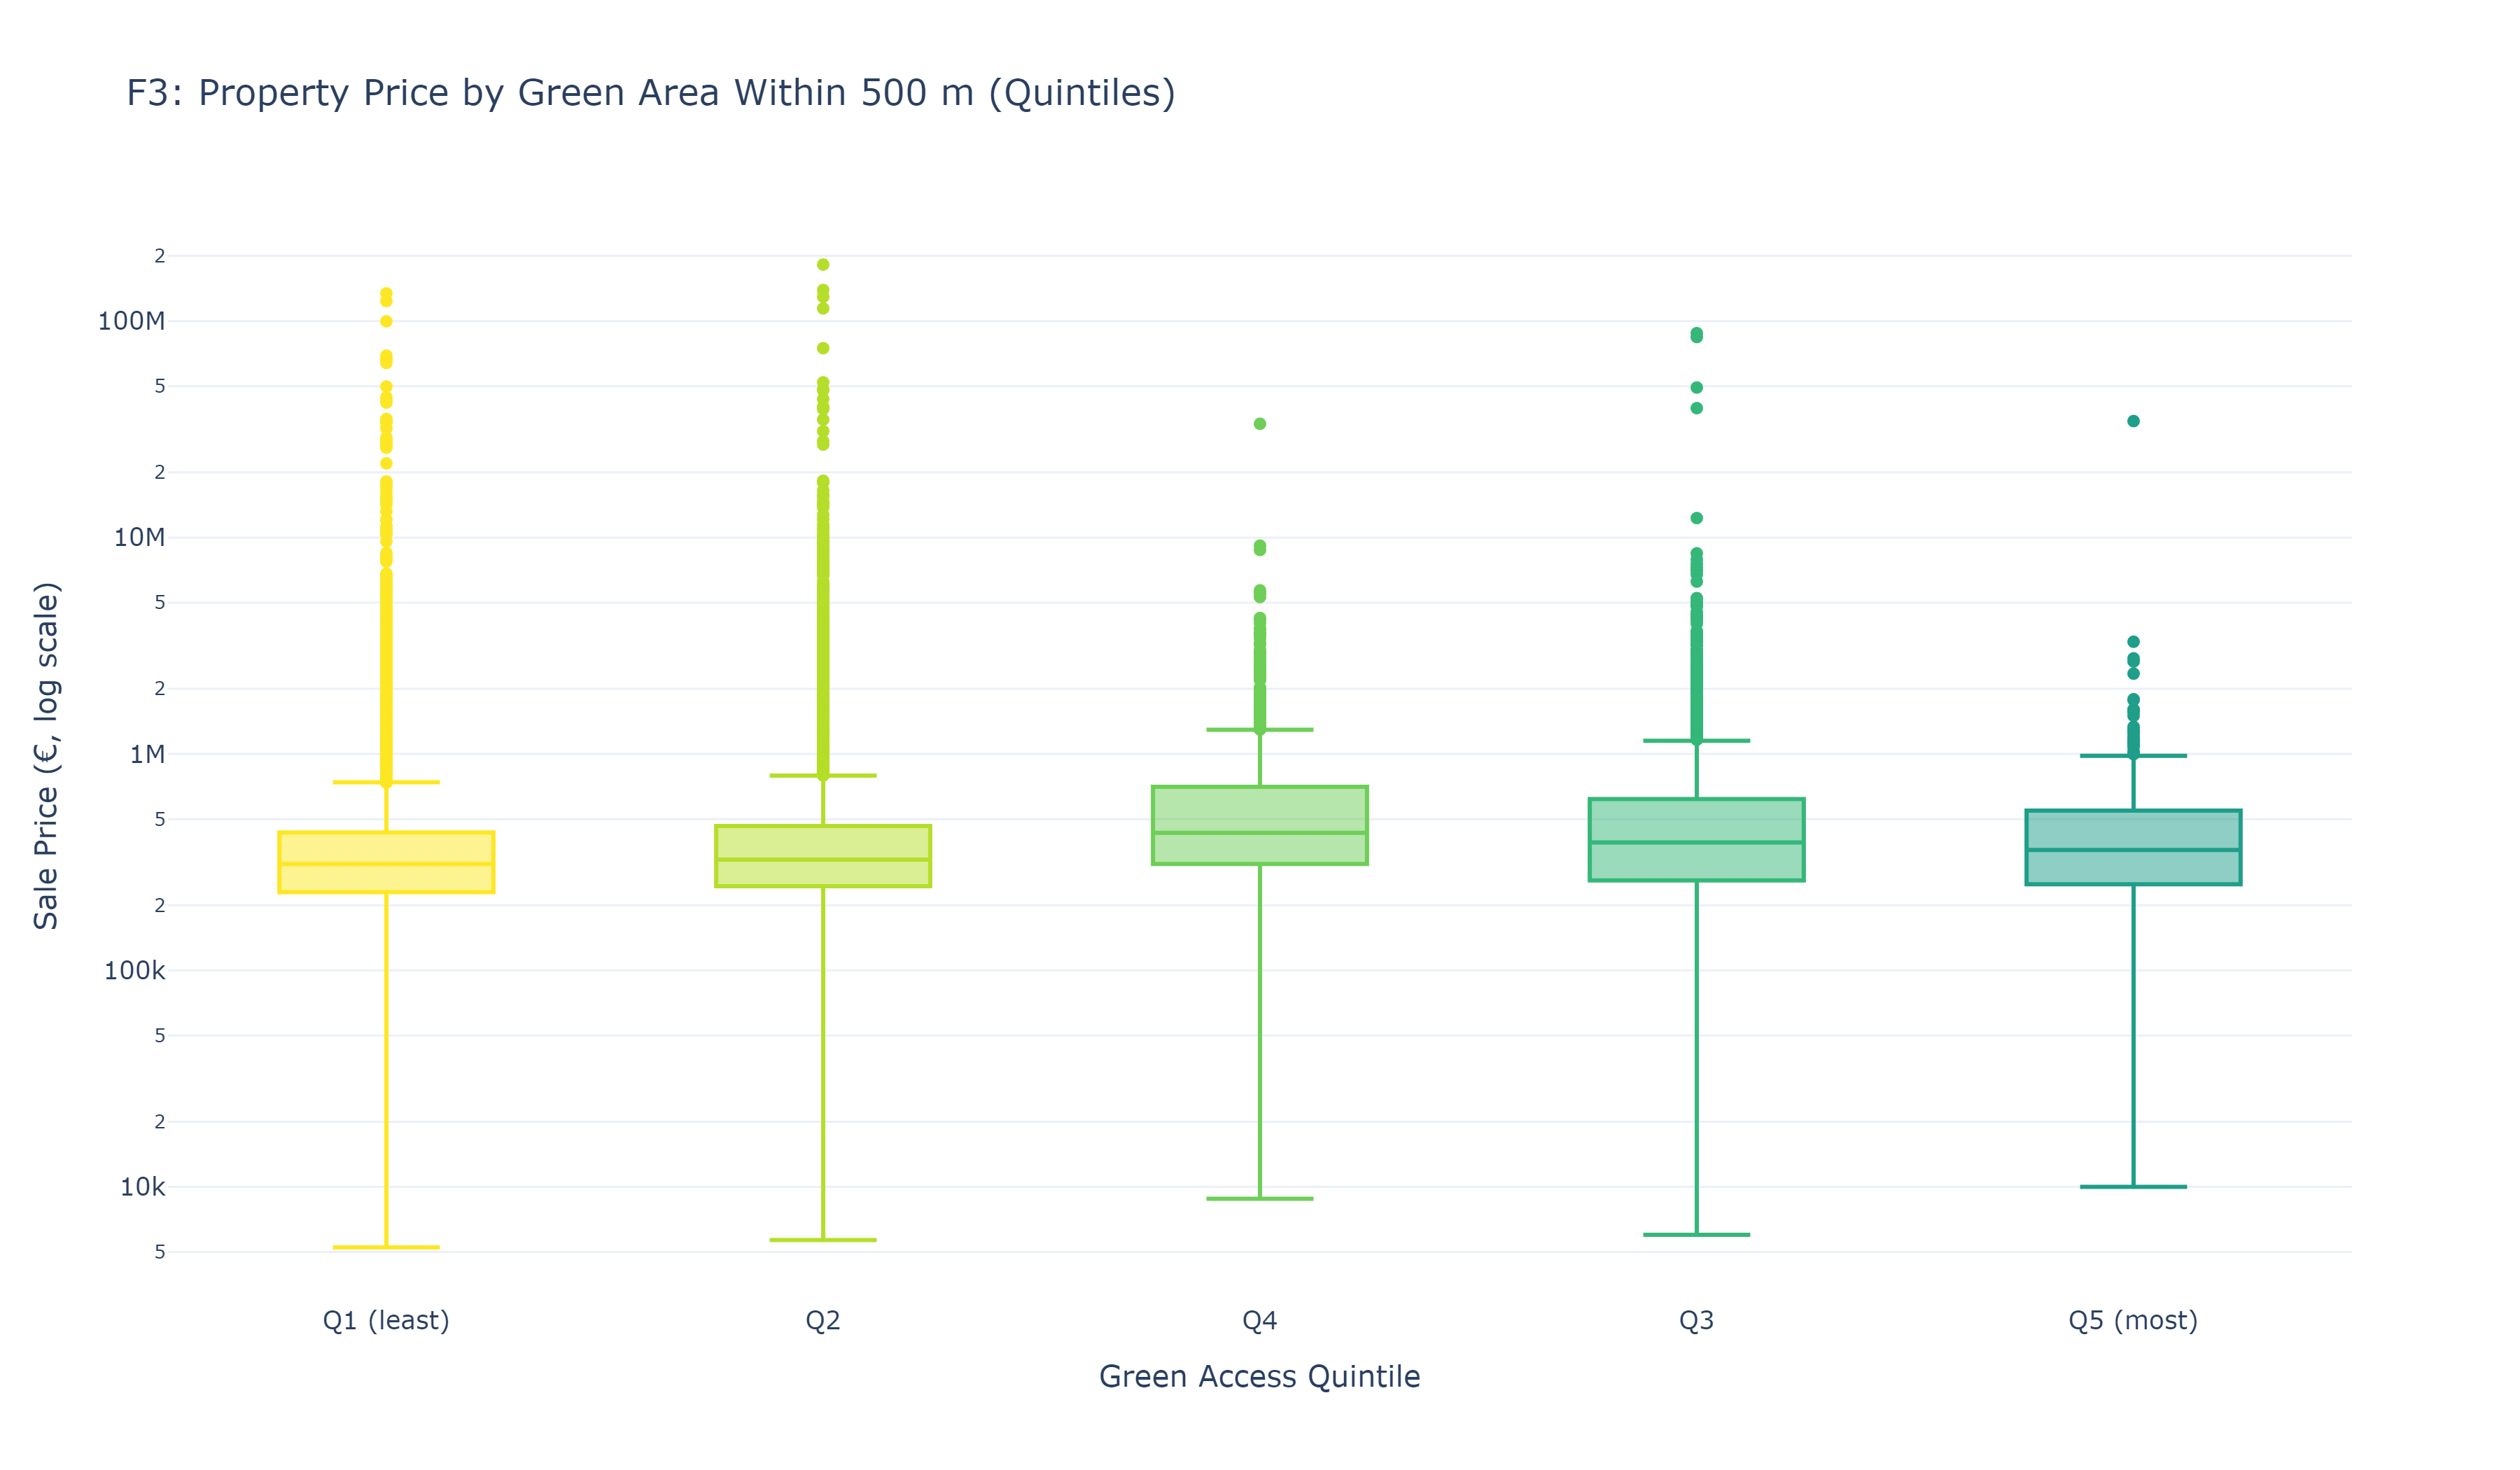
\includegraphics[width=0.95\columnwidth]{figures/F3_plot.png}
\caption{F3 --- Price by green-area-within-500m quintile. Top quintile (Q5)
shows $\sim$15\% higher median price than bottom quintile (Q1).}
\label{fig:f3}
\end{figure}

\begin{figure}[htbp]
\centering
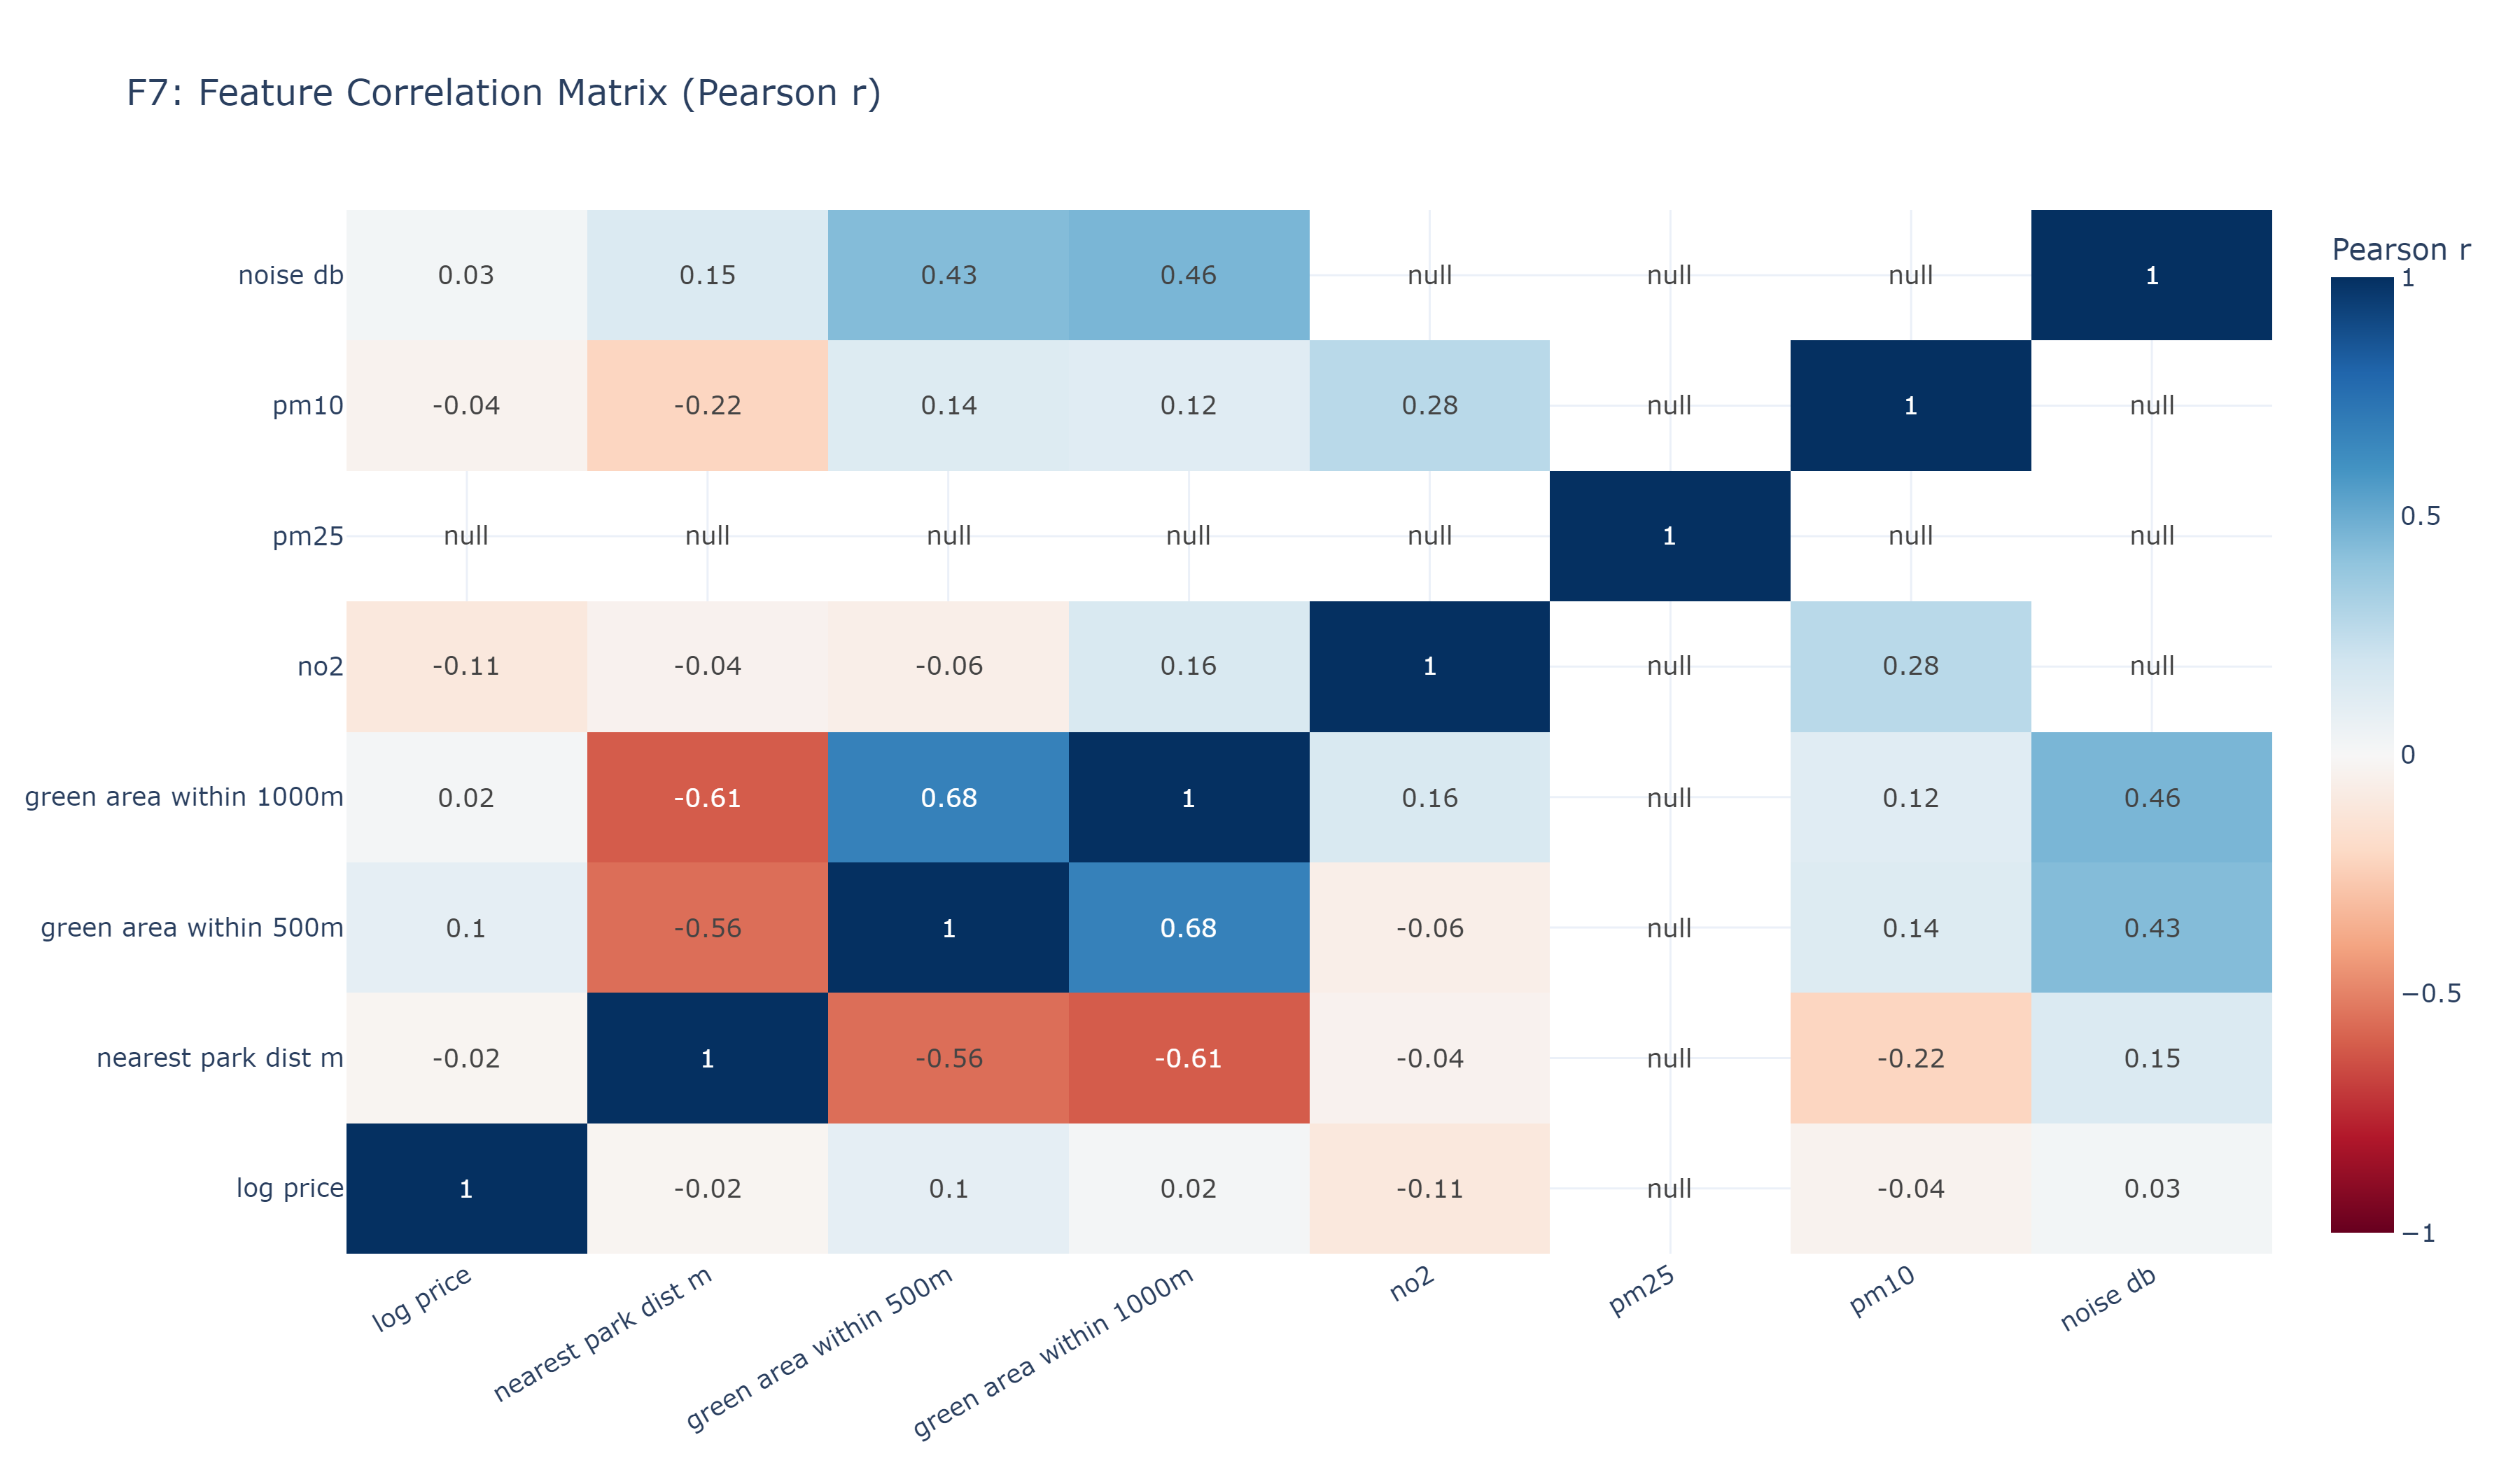
\includegraphics[width=0.95\columnwidth]{figures/F7_plot.png}
\caption{F7 --- Pairwise Pearson correlation heatmap. Green area within
500\,m shows the strongest positive correlation with log-price ($r = 0.095$).
Pairwise deletion handles sparse air quality columns.}
\label{fig:f7}
\end{figure}

\subsection{Finding 2: Park Distance Exhibits Spatial Confounding}

Raw Pearson correlation between nearest-park distance and log-price is
$r = -0.024$ ($p < 0.001$): properties closer to parks have slightly higher
prices. However, the OLS coefficient on $\ln(1 + d_{\text{park}})$ is
\emph{positive} ($\hat{\beta} = 0.075$, $p < 0.001$; Fig.~\ref{fig:f8}).
This sign reversal reflects spatial confounding: Dublin~4, 6, and
14---affluent postal districts---contain large parks (Herbert Park, Marlay
Park) at moderate distance, while inner-city Dublin~1 and~7 have small
parks close to lower-priced properties. These findings corroborate
Jim and Chen~\cite{jimchen2006}, who observed similar confounding in
Guangzhou.

\begin{figure}[htbp]
\centering
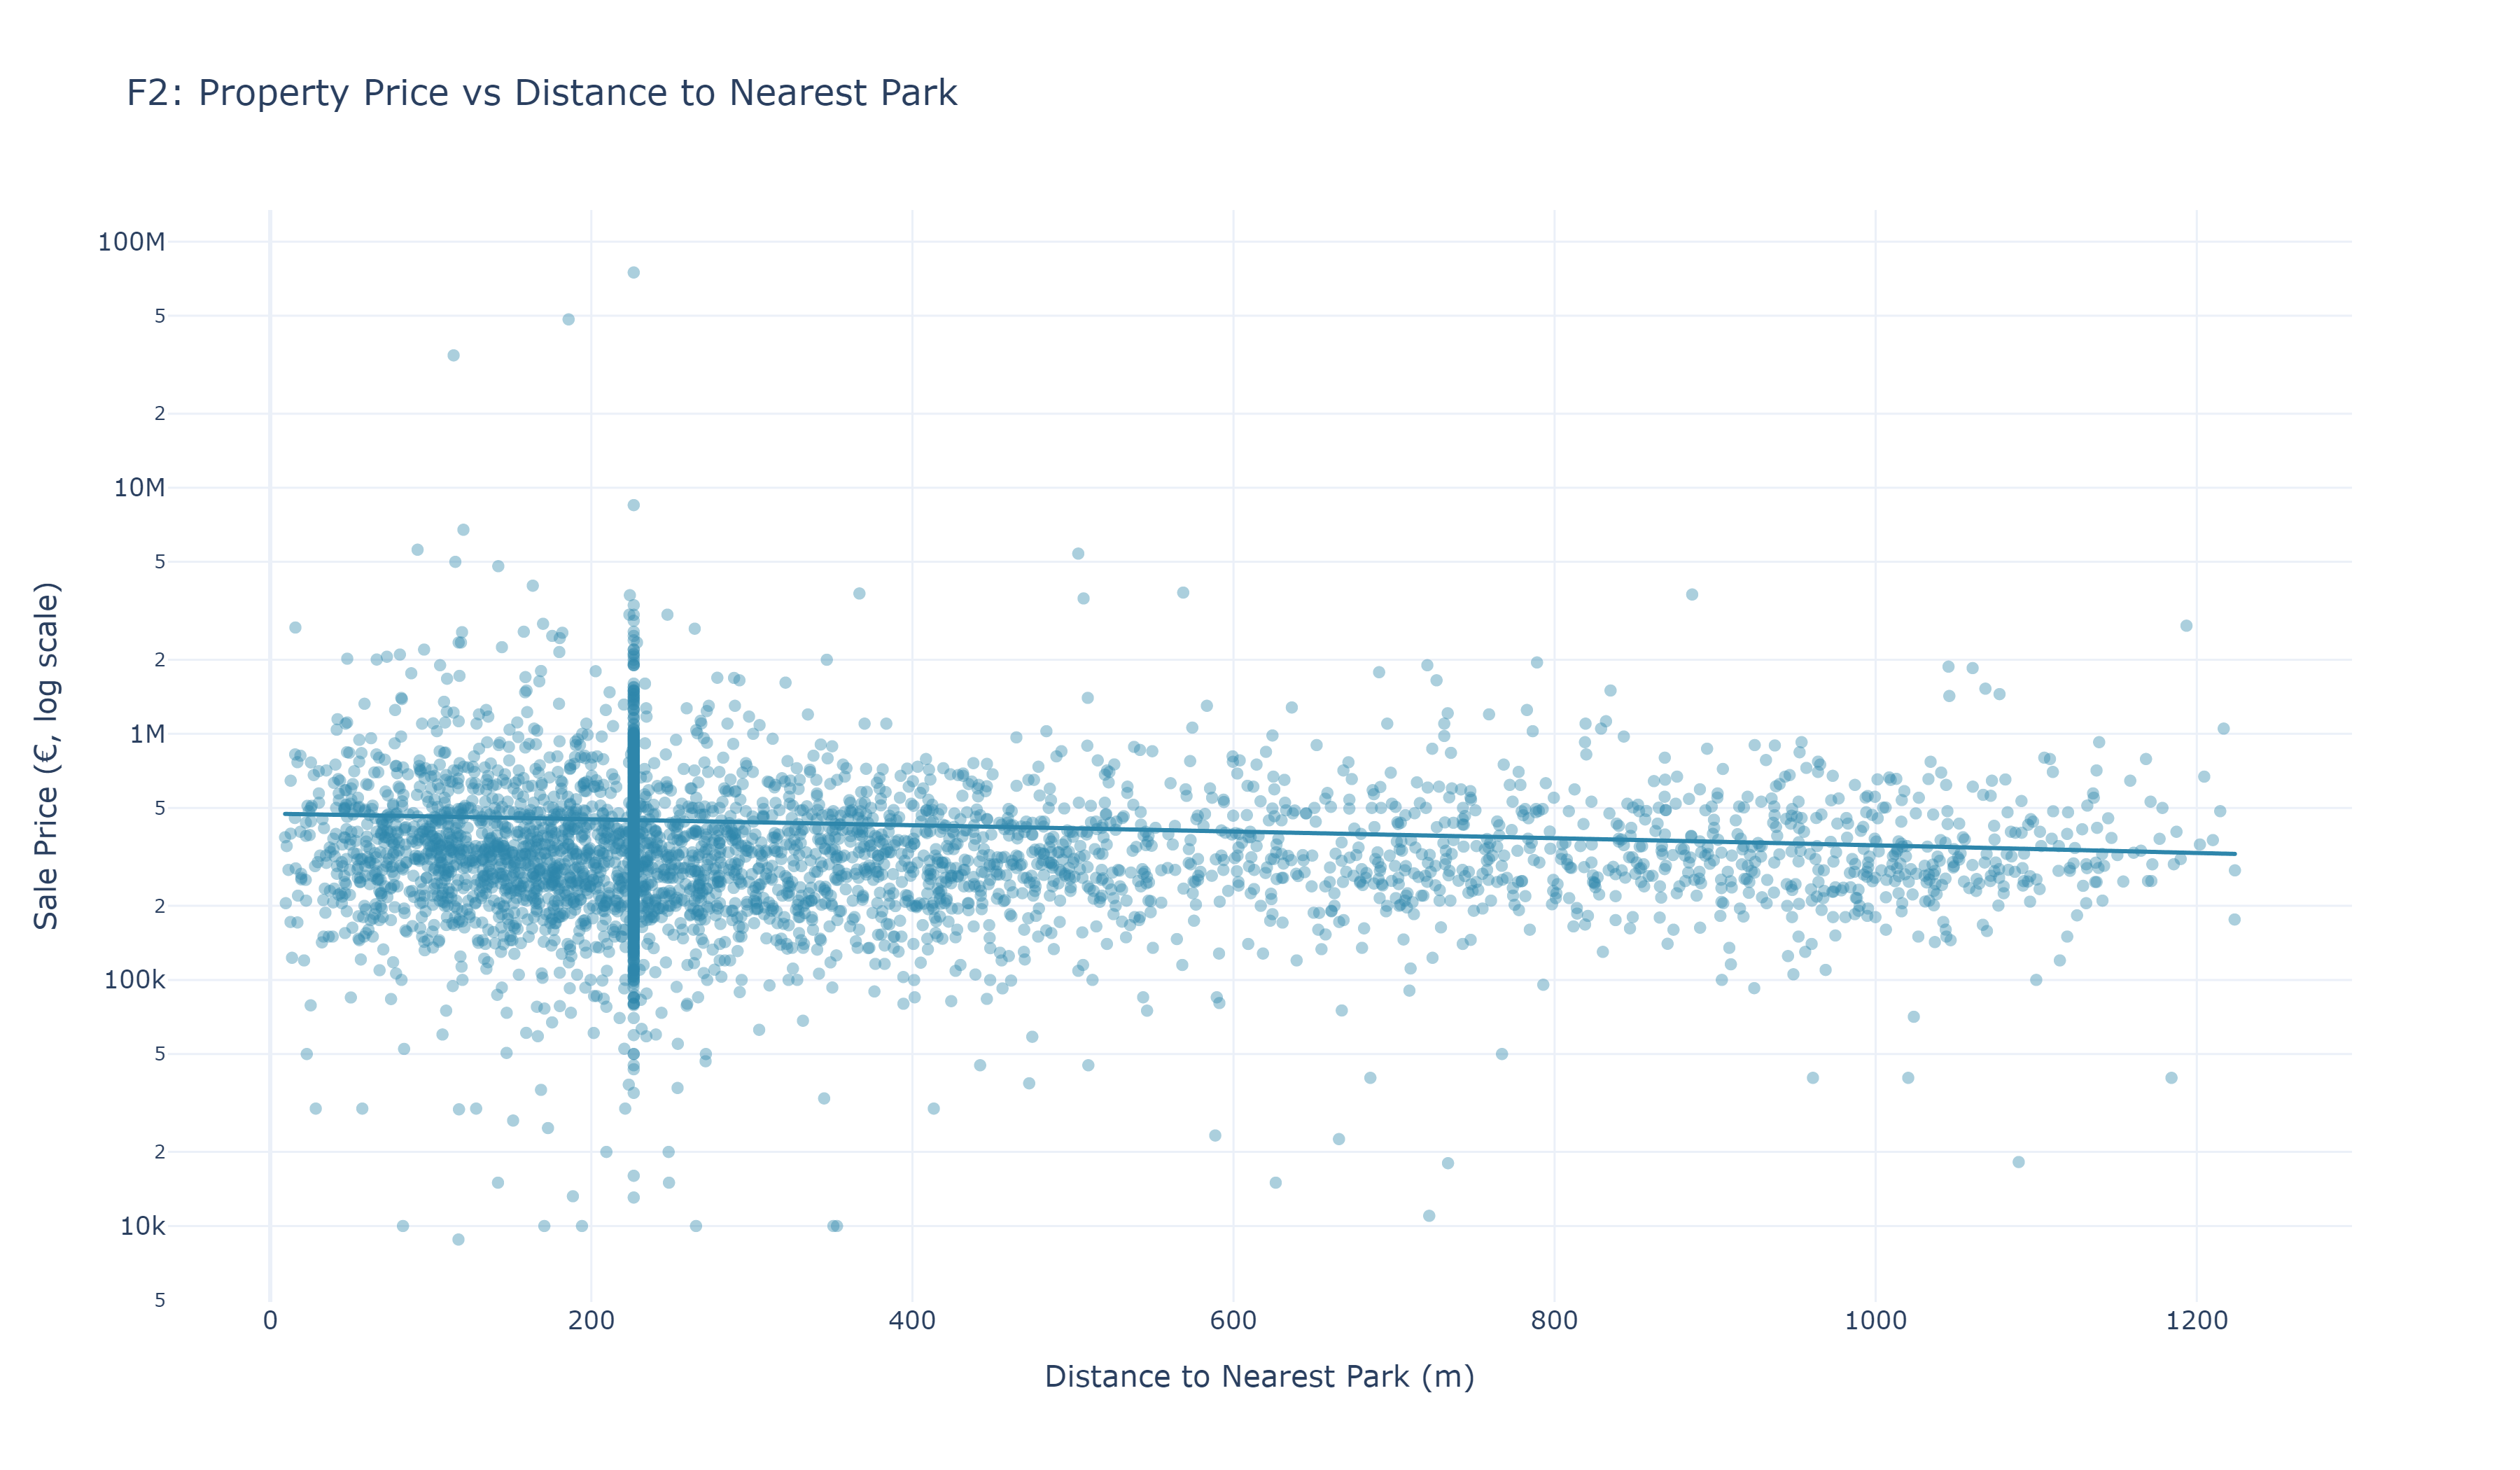
\includegraphics[width=0.95\columnwidth]{figures/F2_plot.png}
\caption{F2 --- Price vs distance to nearest park. The upward OLS trendline
reflects spatial confounding from affluent outer suburbs.}
\label{fig:f2}
\end{figure}

\subsection{Finding 3: NO$_2$ Shows Significant Negative Association}

Among the 20{,}853 properties with matched annual NO$_2$ readings
(2018--2020), the OLS coefficient is $\hat{\beta}_{\text{NO}_2} = -0.010$
($p < 0.001$, 95\% CI: $[-0.012, -0.009]$). Each 1\,\textmu g/m$^3$
increase in annual mean NO$_2$ is associated with a 1.0\% decrease in
property price, holding other variables constant. This directional finding
aligns with Chay and Greenstone~\cite{chaygreenstone2005}. Fig.~\ref{fig:f5}
shows the bivariate scatter, and Fig.~\ref{fig:f4} maps NO$_2$
geographically.

\begin{figure}[htbp]
\centering
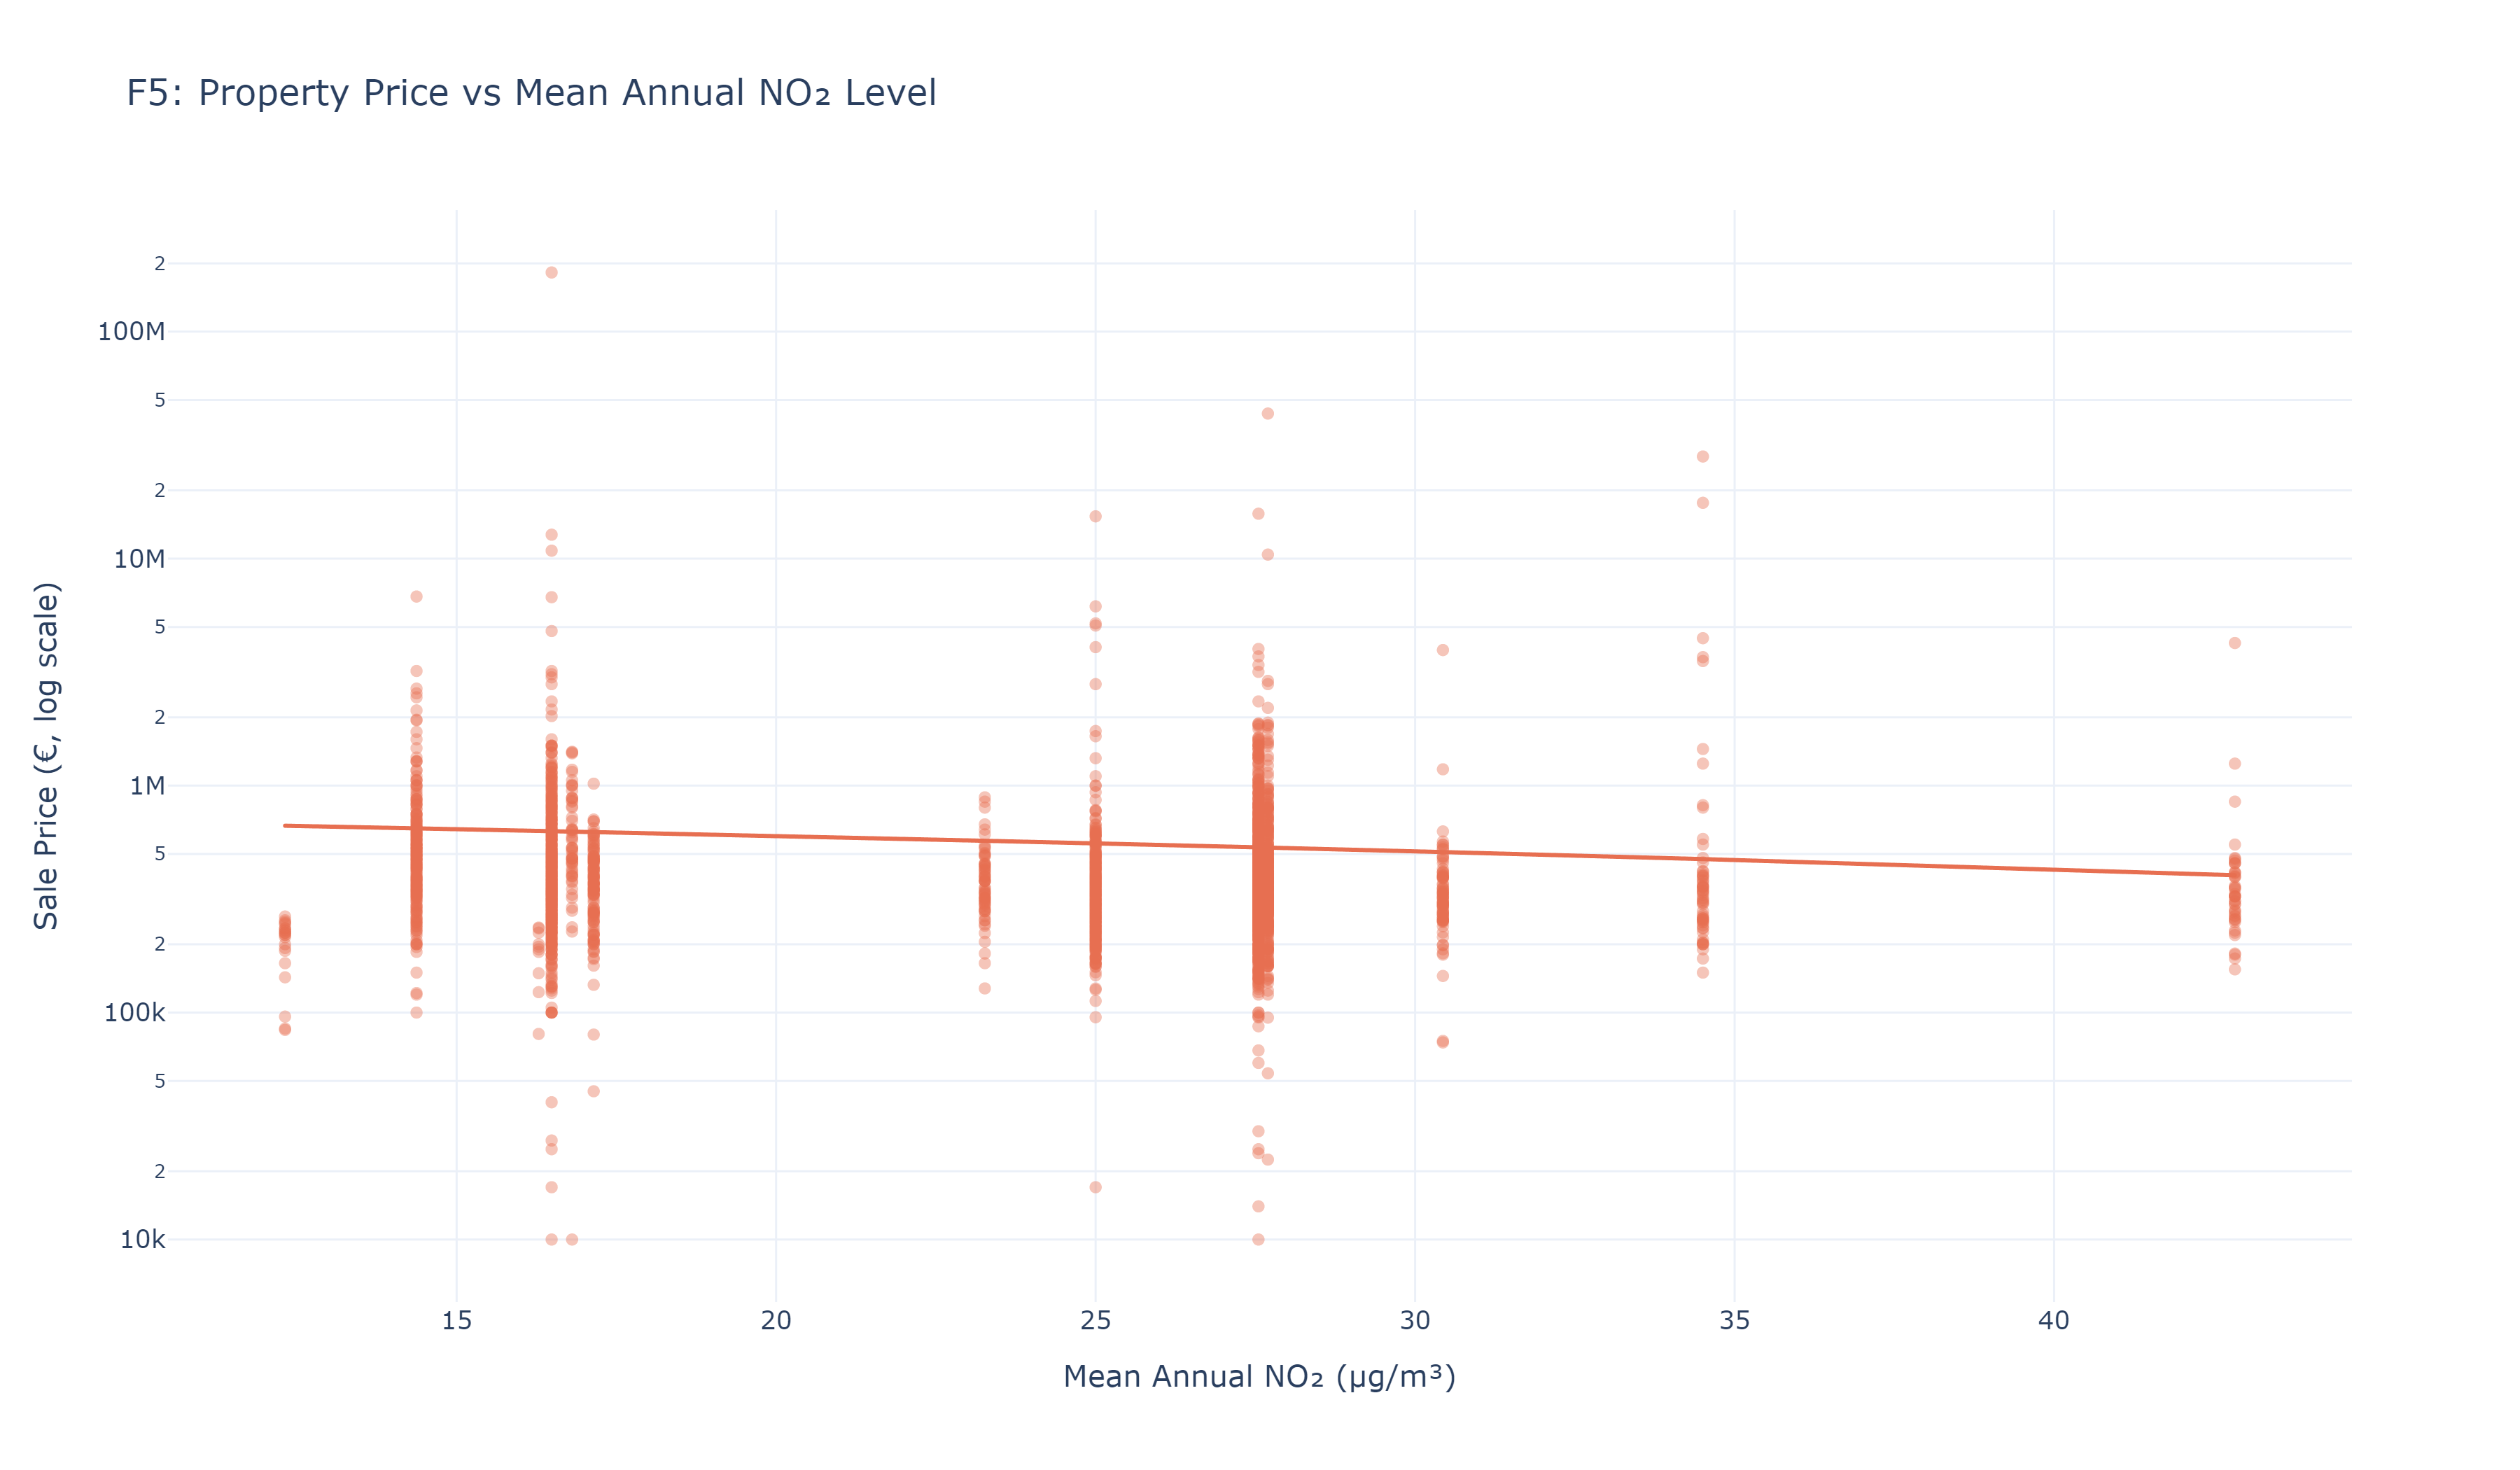
\includegraphics[width=0.95\columnwidth]{figures/F5_plot.png}
\caption{F5 --- Price vs mean annual NO$_2$. Negative trendline confirms
higher NO$_2$ associates with lower prices in the matched subsample.}
\label{fig:f5}
\end{figure}

\begin{figure}[htbp]
\centering
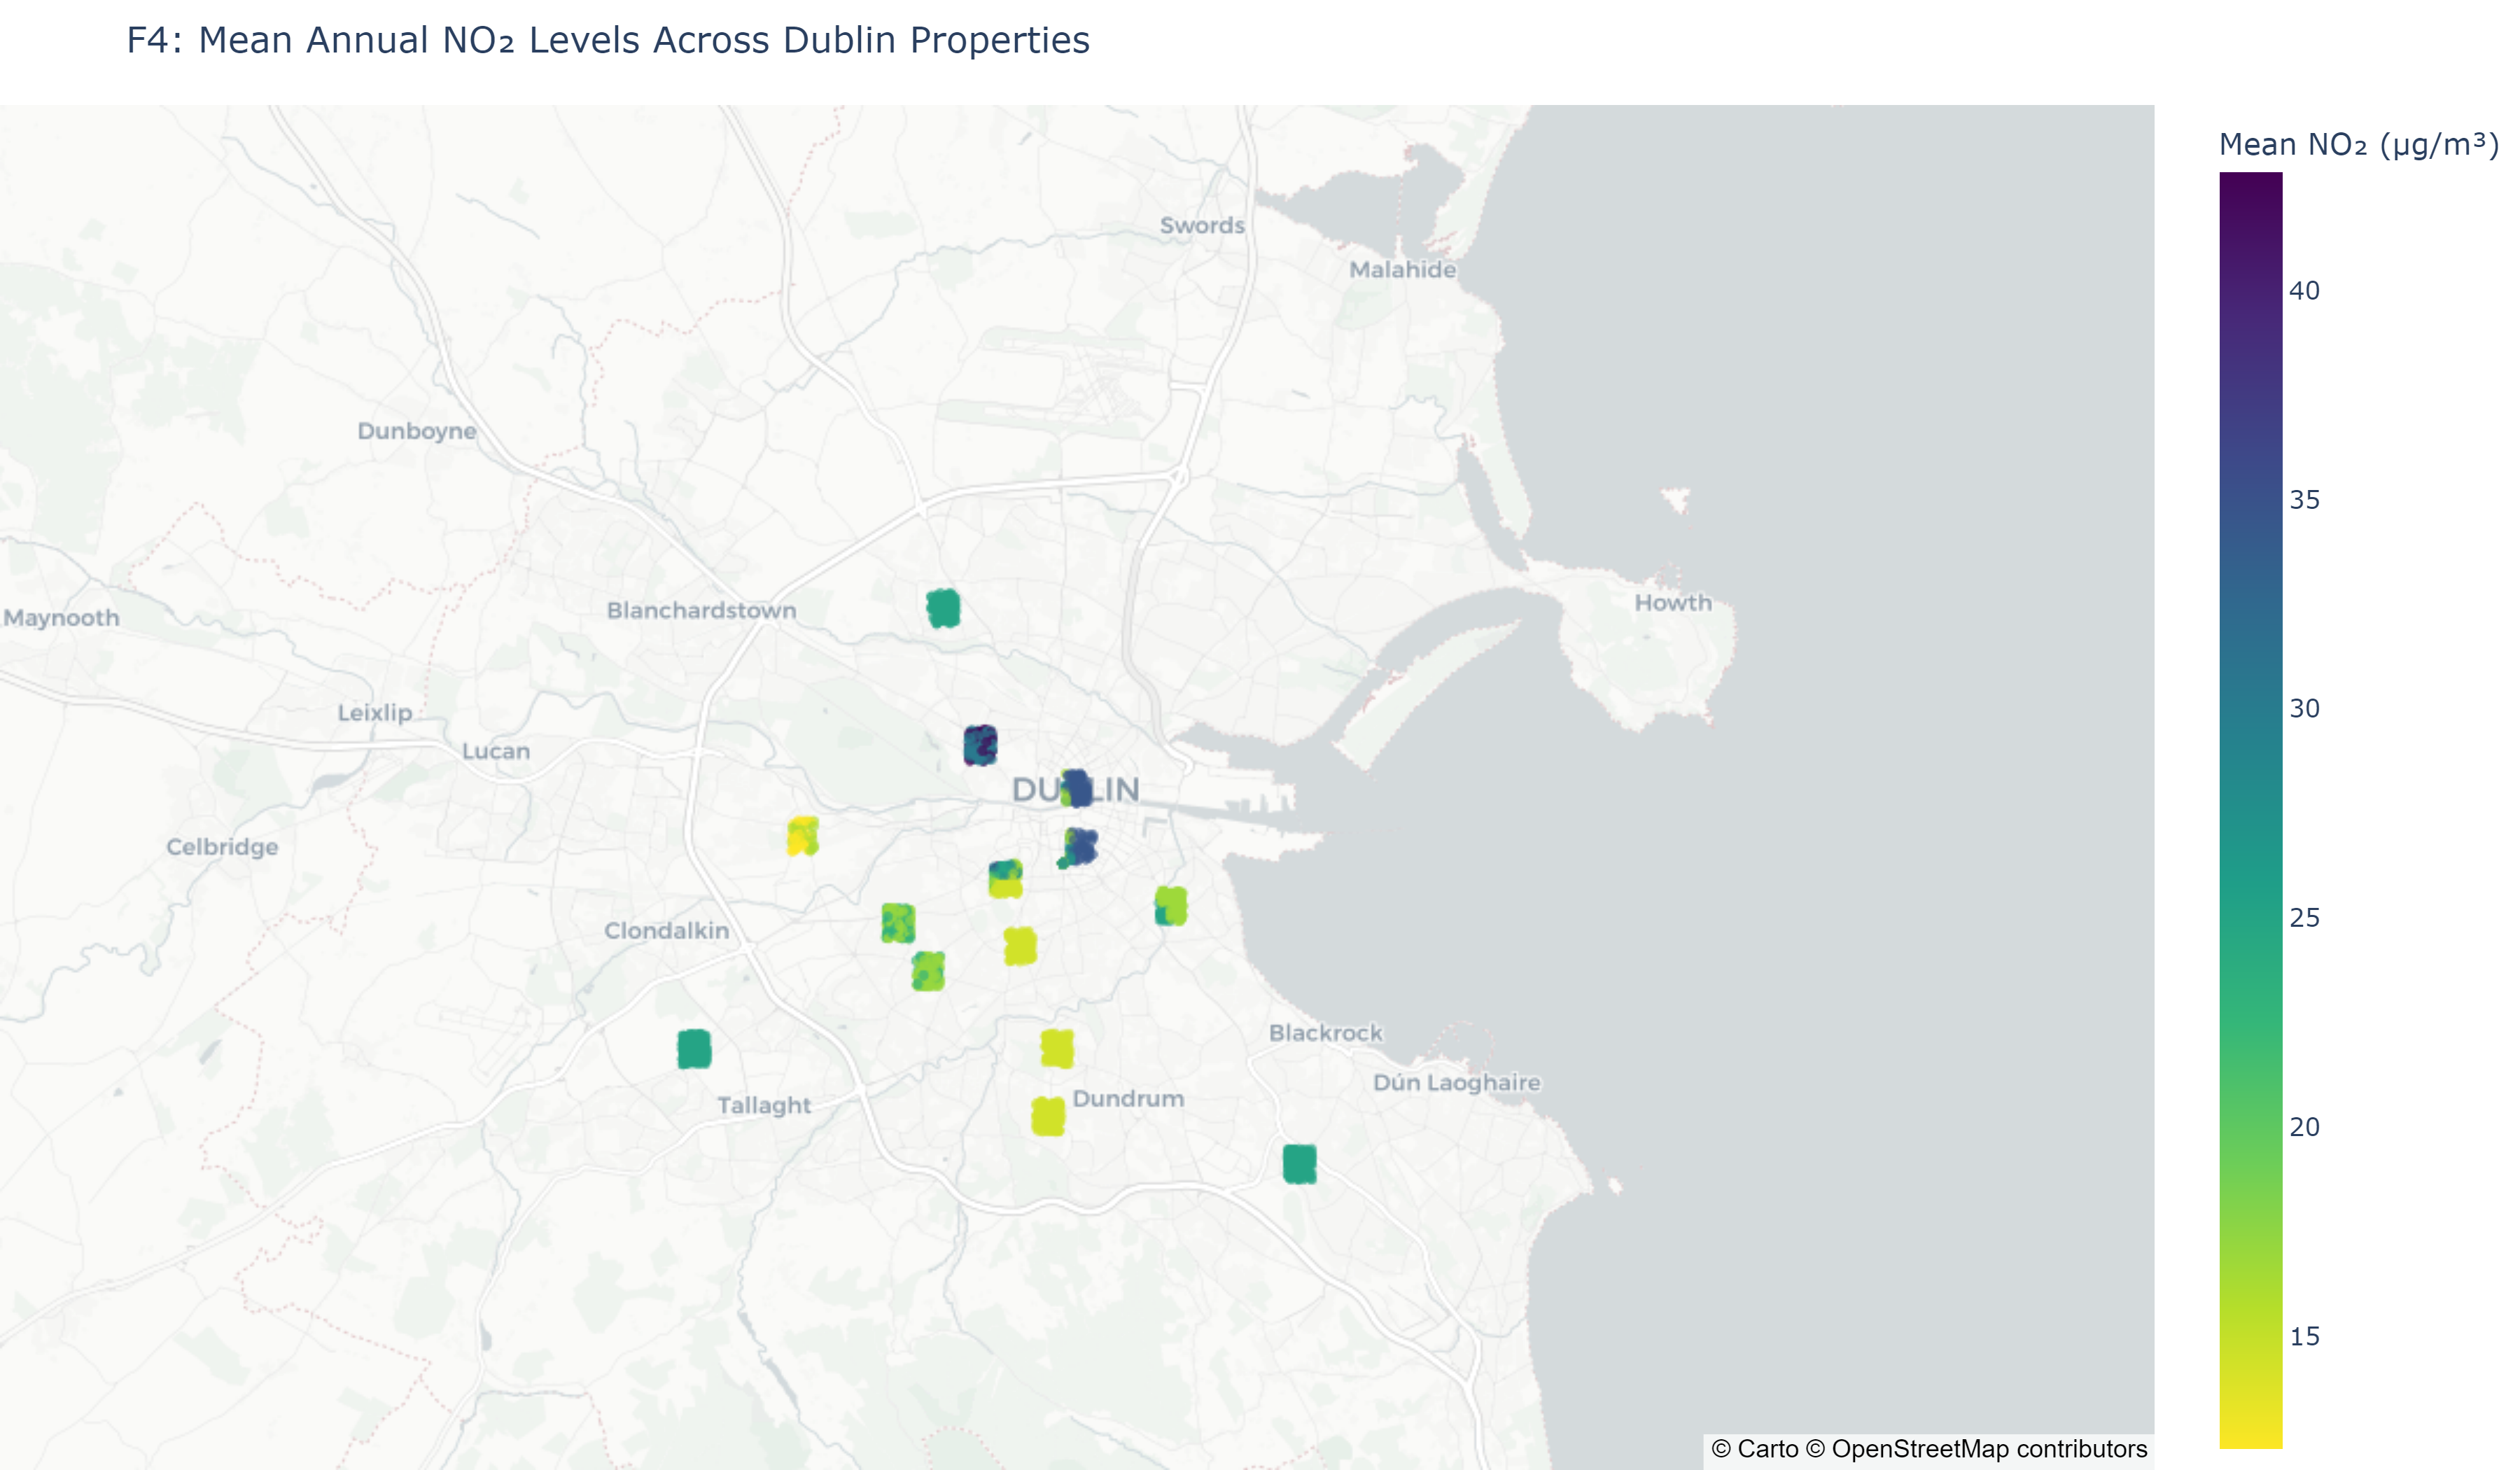
\includegraphics[width=0.95\columnwidth]{figures/F4_no2_map.png}
\caption{F4 --- NO$_2$ by property location. Warmer colours = higher
mean annual NO$_2$ (\textmu g/m$^3$). Coverage concentrated in inner city.}
\label{fig:f4}
\end{figure}

\begin{figure}[htbp]
\centering
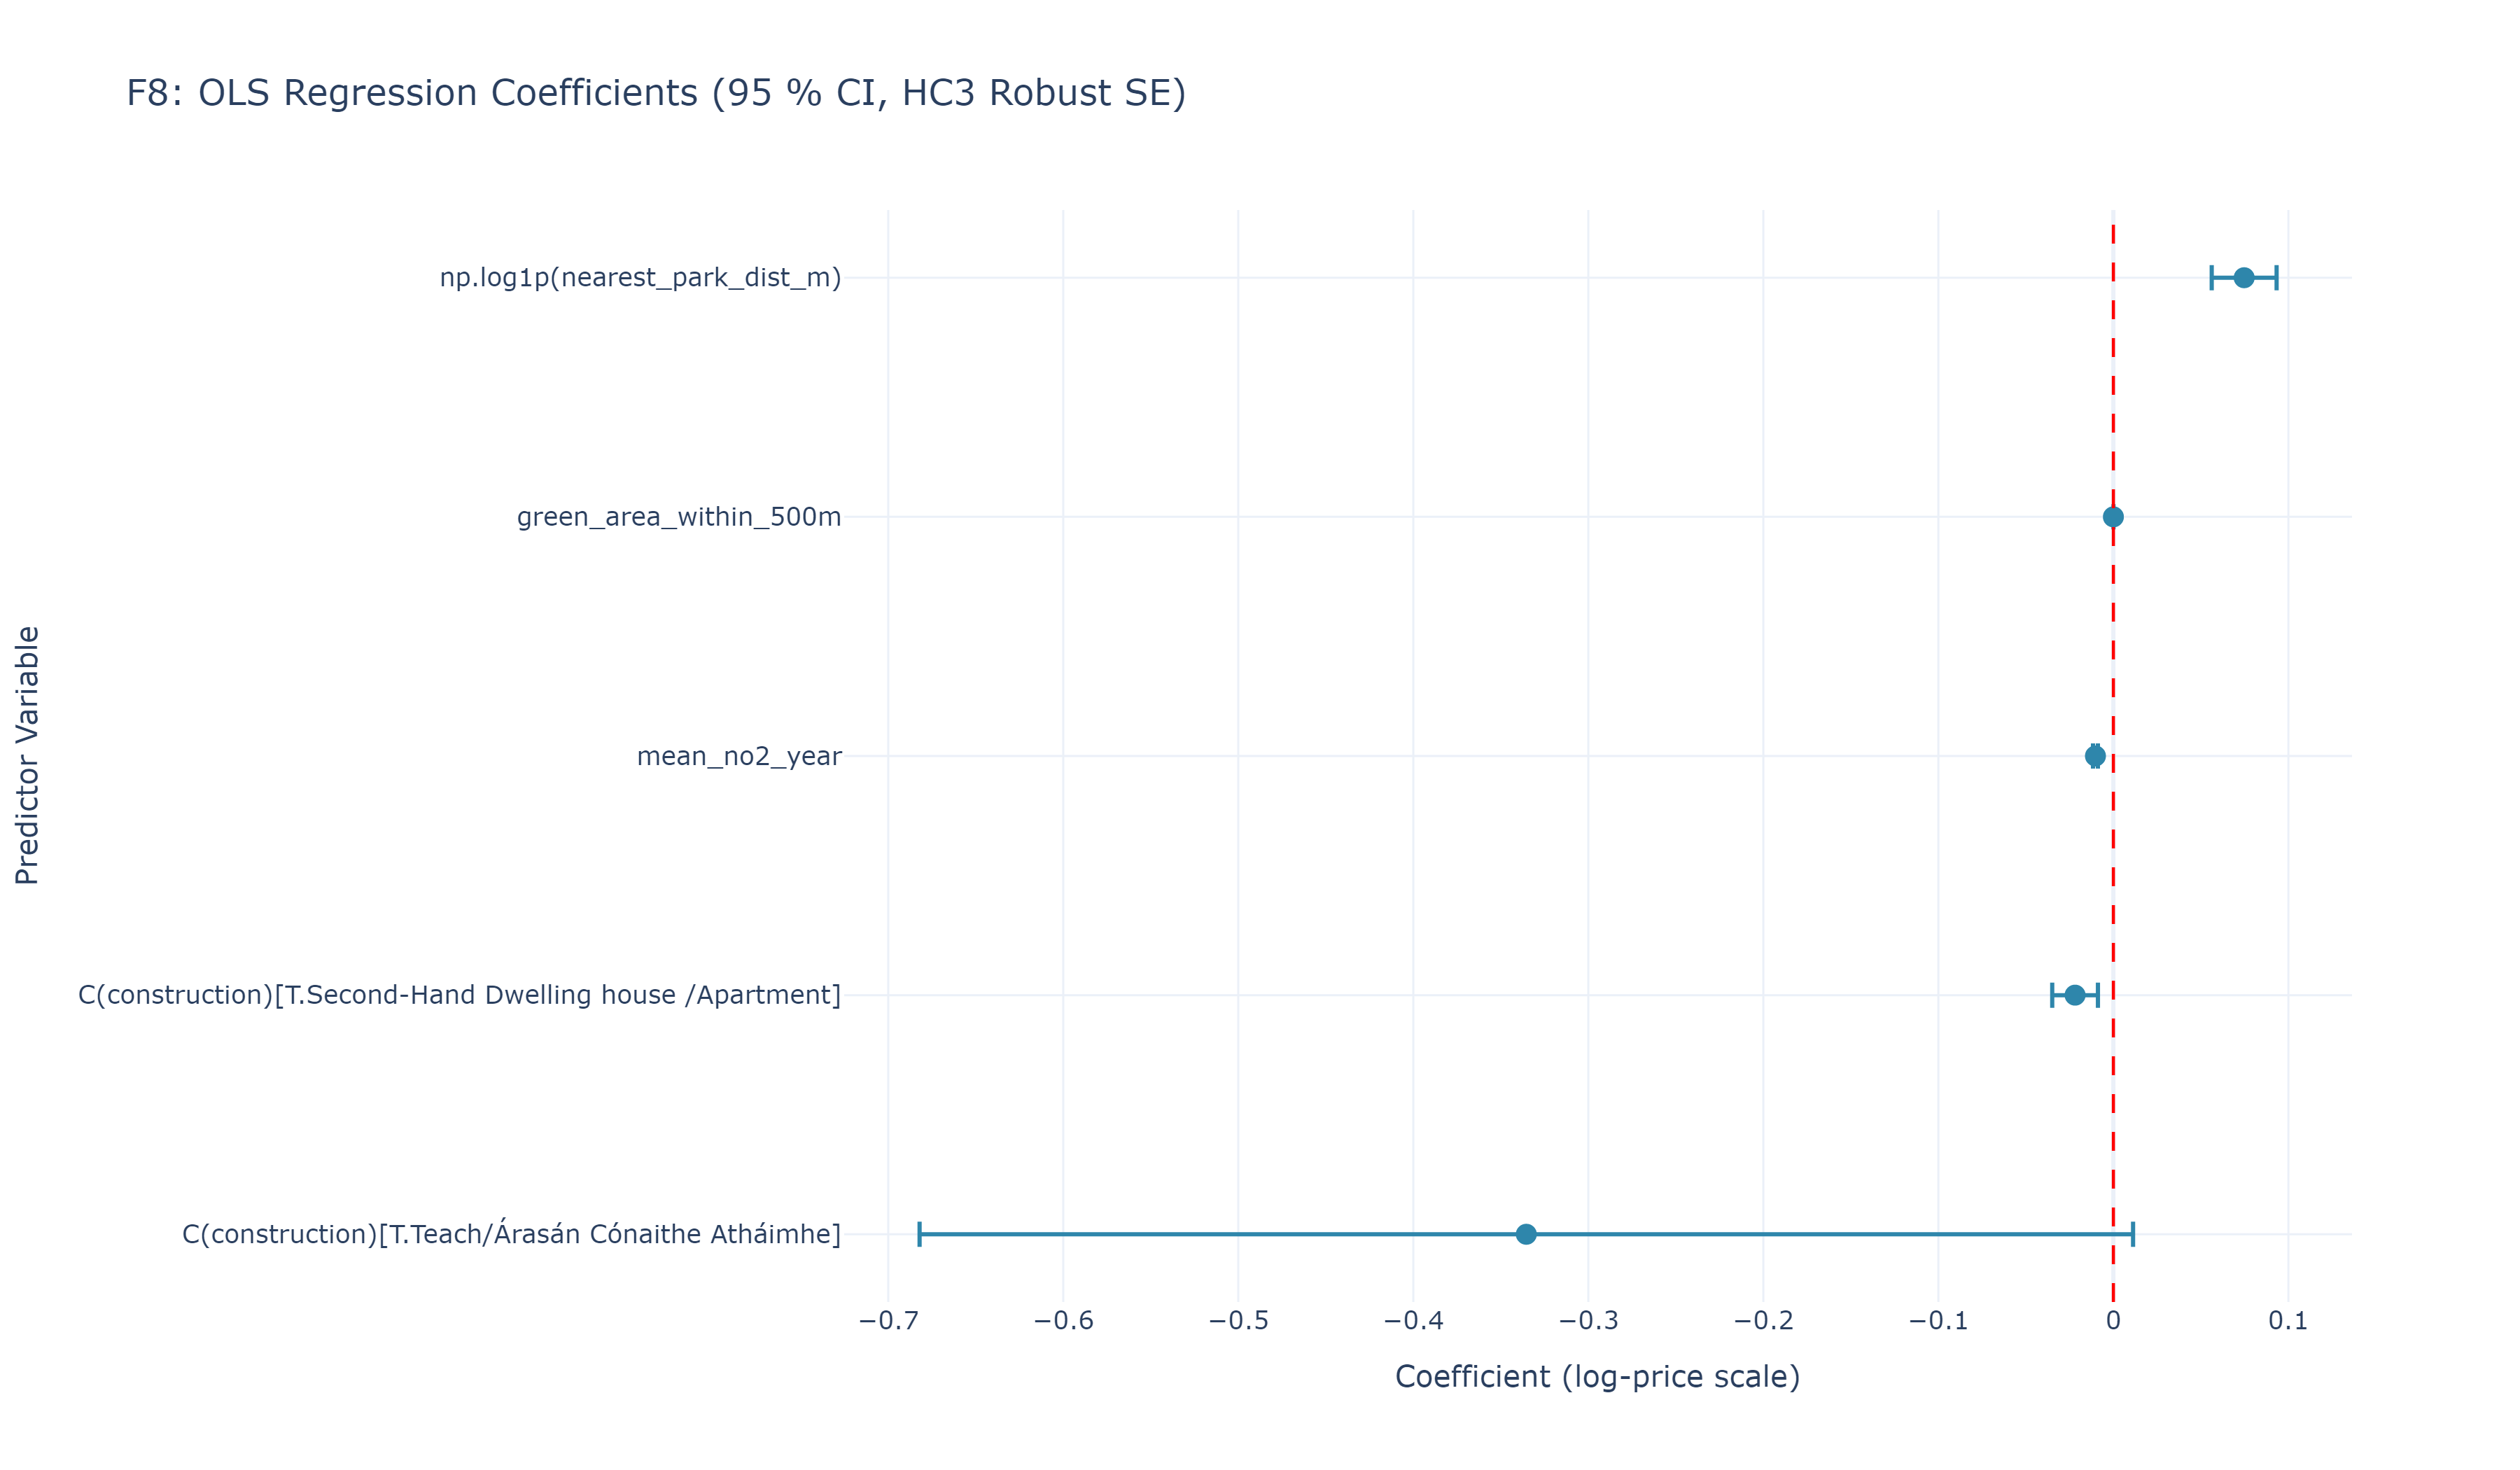
\includegraphics[width=0.95\columnwidth]{figures/F8_plot.png}
\caption{F8 --- OLS forest plot with 95\% CIs (HC3 robust SE). Green area
and NO$_2$ are statistically significant; year and construction type are
controls.}
\label{fig:f8}
\end{figure}

\subsection{Finding 4: Green Premium Gap Widens Over Time}

The temporal analysis (Fig.~\ref{fig:f6}) shows the median price gap between
greenest and least green quintiles grows from \texteuro15{,}000 in 2015 to
\texteuro42{,}000 in 2019, contracting in 2020 (COVID-related transaction
drop). This answers Research Question~4 and aligns with Seya et
al.~\cite{seya2020}.

\begin{figure}[htbp]
\centering
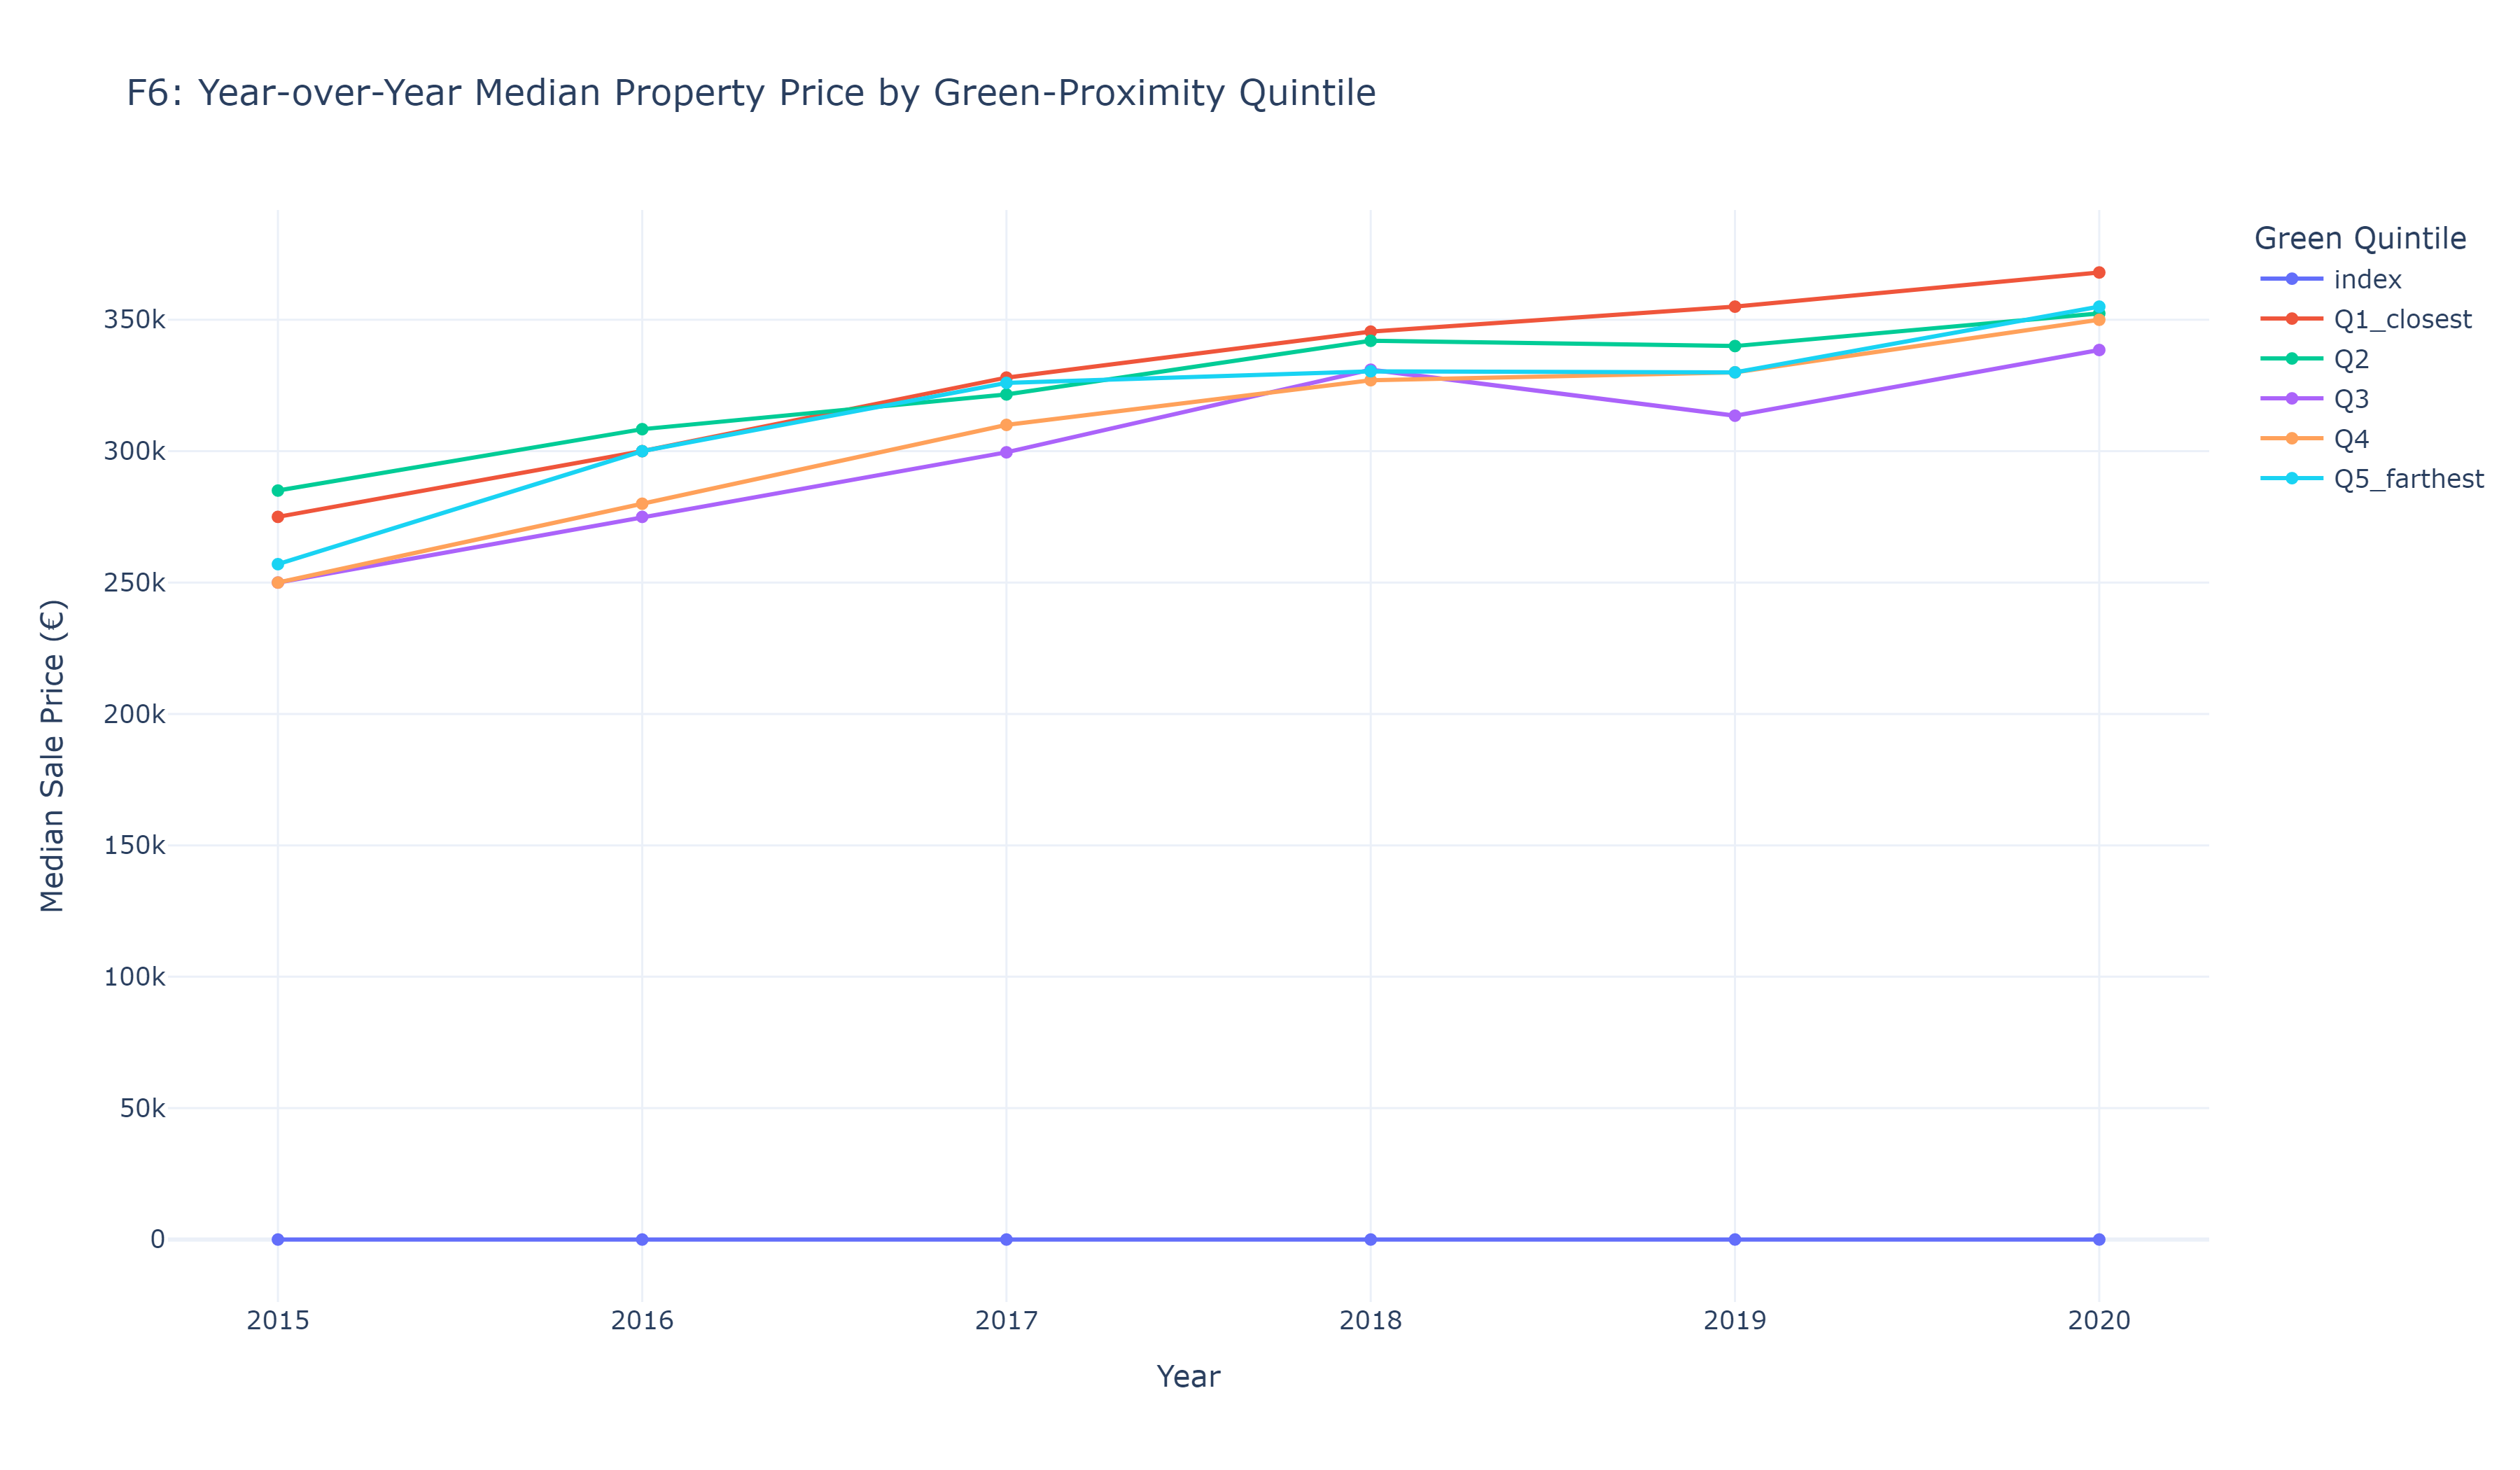
\includegraphics[width=0.95\columnwidth]{figures/F6_plot.png}
\caption{F6 --- Median price by green quintile over time. The gap between
Q1 (most green) and Q5 (least green) widens from 2015 to 2019.}
\label{fig:f6}
\end{figure}

\subsection{Interaction Effect and Model Fit}

The interaction term $\ln(1+d_{\text{park}}) \times \text{NO}_2$ has
coefficient $-0.0014$ ($p = 0.138$), not significant at 5\%. No evidence
of synergistic interaction between green proximity and air quality
(Research Question~3).

The main OLS achieves adjusted $R^2 = 0.019$ with HC3 robust SE. This is
low but expected given postcode-centroid geocoding, absence of structural
features (bedrooms, floor area), and limited AQ coverage. The model is
presented for association interpretation, not prediction.
Table~\ref{tab:ols} summarises key coefficients.

\begin{table}[htbp]
\centering
\caption{OLS Regression Coefficients (Main Model)}
\label{tab:ols}
\begin{tabular}{lrrr}
\toprule
\textbf{Variable} & \textbf{Coeff.} & \textbf{95\% CI} & \textbf{p} \\
\midrule
Intercept & 12.633 & [12.51, 12.76] & $<$0.001 \\
$\ln(1+d_{\text{park}})$ & 0.075 & [0.056, 0.093] & $<$0.001 \\
Green area (500m) & 8.9e-7 & [6.5e-7, 1.1e-6] & $<$0.001 \\
Mean NO$_2$ & $-$0.010 & [$-$0.012, $-$0.009] & $<$0.001 \\
Year 2020 & $-$0.031 & [$-$0.050, $-$0.010] & 0.003 \\
Second-hand & $-$0.022 & [$-$0.035, $-$0.009] & 0.001 \\
\bottomrule
\multicolumn{4}{l}{\small Adj.\ $R^2 = 0.019$; $n = 20{,}853$; HC3 robust SE.}
\end{tabular}
\end{table}

% ============================================================
\section{Conclusions and Future Work}
\label{sec:conclusion}
% ============================================================

This paper demonstrates a reproducible end-to-end pipeline from open data
ingestion through spatial enrichment to interactive visualisation, integrating
three heterogeneous datasets across two database systems. Four key findings
emerge:

\begin{enumerate}
  \item \textbf{Green area within 500\,m} carries a positive, statistically
        significant price association ($r = 0.095$, $p < 0.001$),
        with the top quintile commanding $\sim$15\% higher median prices.
  \item \textbf{Nearest-park distance} is confounded by district-level
        spatial heterogeneity, producing a counterintuitive positive OLS
        coefficient requiring spatial fixed effects for causal interpretation.
  \item \textbf{NO$_2$} shows a significant negative association ($-1.0\%$
        per \textmu g/m$^3$), consistent with hedonic air quality literature.
  \item \textbf{The green premium gap widens} from 2015 to 2019,
        suggesting increasing market valuation of environmental amenities.
\end{enumerate}

\textbf{Limitations.} Postcode-centroid geocoding provides district-level
rather than address-level precision. Air quality coverage is limited to
2018--2020 for the matched subsample. No structural property controls
(floor area, bedrooms) are available in the PSRA register. The OLS
framework does not establish causality.

\textbf{Future work} should (i)~apply address-level geocoding using the
Eircode routing key database; (ii)~implement difference-in-differences
exploiting air quality station installation dates; (iii)~integrate CSO
Census~2022 socioeconomic controls; and (iv)~extend to 2022--2025 data.

% ============================================================
\section*{Acknowledgements}
% ============================================================

Data sourced from the Property Services Regulatory Authority, Dublin City
Council Sonitus air quality monitoring network, and Dublin local authority
open data portals via \texttt{data.smartdublin.ie}.

% ============================================================
\bibliographystyle{IEEEtran}
\bibliography{references}

\end{document}
